% **************************************************************************************************************
% A Classic Thesis Style
% An Homage to The Elements of Typographic Style
%
% Copyright (C) 2018 André Miede and Ivo Pletikosić
%
% If you like the style then I would appreciate a postcard. My address
% can be found in the file ClassicThesis.pdf. A collection of the
% postcards I received so far is available online at
% http://postcards.miede.de
%
% License:
% This program is free software; you can redistribute it and/or modify
% it under the terms of the GNU General Public License as published by
% the Free Software Foundation; either version 2 of the License, or
% (at your option) any later version.
%
% This program is distributed in the hope that it will be useful,
% but WITHOUT ANY WARRANTY; without even the implied warranty of
% MERCHANTABILITY or FITNESS FOR A PARTICULAR PURPOSE.  See the
% GNU General Public License for more details.
%
% You should have received a copy of the GNU General Public License
% along with this program; see the file COPYING.  If not, write to
% the Free Software Foundation, Inc., 59 Temple Place - Suite 330,
% Boston, MA 02111-1307, USA.
%
% PLEASE SEE ALSO THE AUTHORS' NOTE REGARDING THIS LICENSE
% IN THE DOCUMENTATION (ClassicThesis.pdf --> Chapter 1 / Chapter01.tex)
% **************************************************************************************************************
\RequirePackage{silence} % :-\
    \WarningFilter{scrreprt}{Usage of package `titlesec'}
    %\WarningFilter{scrreprt}{Activating an ugly workaround}
    \WarningFilter{titlesec}{Non standard sectioning command detected}
\documentclass[ twoside,openright,titlepage,numbers=noenddot,%1headlines,
                headinclude,footinclude,cleardoublepage=empty,abstract=on,
                BCOR=5mm,paper=a4,fontsize=11pt
                ]{scrreprt}

%********************************************************************
% Note: Make all your adjustments in here
%*******************************************************
% ****************************************************************************************************
% classicthesis-config.tex
% formerly known as loadpackages.sty, classicthesis-ldpkg.sty, and classicthesis-preamble.sty
% Use it at the beginning of your ClassicThesis.tex, or as a LaTeX Preamble
% in your ClassicThesis.{tex,lyx} with % ****************************************************************************************************
% classicthesis-config.tex
% formerly known as loadpackages.sty, classicthesis-ldpkg.sty, and classicthesis-preamble.sty
% Use it at the beginning of your ClassicThesis.tex, or as a LaTeX Preamble
% in your ClassicThesis.{tex,lyx} with % ****************************************************************************************************
% classicthesis-config.tex
% formerly known as loadpackages.sty, classicthesis-ldpkg.sty, and classicthesis-preamble.sty
% Use it at the beginning of your ClassicThesis.tex, or as a LaTeX Preamble
% in your ClassicThesis.{tex,lyx} with \input{classicthesis-config}
% ****************************************************************************************************
% If you like the classicthesis, then I would appreciate a postcard.
% My address can be found in the file ClassicThesis.pdf. A collection
% of the postcards I received so far is available online at
% http://postcards.miede.de
% ****************************************************************************************************


% ****************************************************************************************************
% 0. Set the encoding of your files. UTF-8 is the only sensible encoding nowadays. If you can't read
% äöüßáéçèê∂åëæƒÏ€ then change the encoding setting in your editor, not the line below. If your editor
% does not support utf8 use another editor!
% ****************************************************************************************************
\PassOptionsToPackage{utf8}{inputenc}
  \usepackage{inputenc}

\PassOptionsToPackage{T1}{fontenc} % T2A for cyrillics
  \usepackage{fontenc}


% ****************************************************************************************************
% 1. Configure classicthesis for your needs here, e.g., remove "drafting" below
% in order to deactivate the time-stamp on the pages
% (see ClassicThesis.pdf for more information):
% ****************************************************************************************************
\PassOptionsToPackage{
  drafting=true,    % print version information on the bottom of the pages
  tocaligned=false, % the left column of the toc will be aligned (no indentation)
  dottedtoc=false,  % page numbers in ToC flushed right
  eulerchapternumbers=true, % use AMS Euler for chapter font (otherwise Palatino)
  linedheaders=false,       % chaper headers will have line above and beneath
  floatperchapter=true,     % numbering per chapter for all floats (i.e., Figure 1.1)
  eulermath=false,  % use awesome Euler fonts for mathematical formulae (only with pdfLaTeX)
  beramono=true,    % toggle a nice monospaced font (w/ bold)
  palatino=true,    % deactivate standard font for loading another one, see the last section at the end of this file for suggestions
  style=classicthesis % classicthesis, arsclassica
}{classicthesis}


% ****************************************************************************************************
% 2. Personal data and user ad-hoc commands (insert your own data here)
% ****************************************************************************************************
\newcommand{\myTitle}{A Classic Thesis Style\xspace}
\newcommand{\mySubtitle}{An Homage to The Elements of Typographic Style\xspace}
\newcommand{\myDegree}{Doktor-Ingenieur (Dr.-Ing.)\xspace}
\newcommand{\myName}{André Miede \& Ivo Pletikosić\xspace}
\newcommand{\myProf}{Put name here\xspace}
\newcommand{\myOtherProf}{Put name here\xspace}
\newcommand{\mySupervisor}{Put name here\xspace}
\newcommand{\myFaculty}{Put data here\xspace}
\newcommand{\myDepartment}{Put data here\xspace}
\newcommand{\myUni}{Put data here\xspace}
\newcommand{\myLocation}{Saarbrücken\xspace}
\newcommand{\myTime}{June 2018\xspace}
\newcommand{\myVersion}{\classicthesis}

% ********************************************************************
% Setup, finetuning, and useful commands
% ********************************************************************
\providecommand{\mLyX}{L\kern-.1667em\lower.25em\hbox{Y}\kern-.125emX\@}
\newcommand{\ie}{i.\,e.}
\newcommand{\Ie}{I.\,e.}
\newcommand{\eg}{e.\,g.}
\newcommand{\Eg}{E.\,g.}
% ****************************************************************************************************


% ****************************************************************************************************
% 3. Loading some handy packages
% ****************************************************************************************************
% ********************************************************************
% Packages with options that might require adjustments
% ********************************************************************
\PassOptionsToPackage{ngerman,american}{babel} % change this to your language(s), main language last
% Spanish languages need extra options in order to work with this template
%\PassOptionsToPackage{spanish,es-lcroman}{babel}
    \usepackage{babel}

\usepackage{csquotes}
\PassOptionsToPackage{%
  %backend=biber,bibencoding=utf8, %instead of bibtex
  backend=bibtex8,bibencoding=ascii,%
  language=auto,%
  style=numeric-comp,%
  %style=authoryear-comp, % Author 1999, 2010
  %bibstyle=authoryear,dashed=false, % dashed: substitute rep. author with ---
  sorting=nyt, % name, year, title
  maxbibnames=10, % default: 3, et al.
  %backref=true,%
  natbib=true % natbib compatibility mode (\citep and \citet still work)
}{biblatex}
    \usepackage{biblatex}

\PassOptionsToPackage{fleqn}{amsmath}       % math environments and more by the AMS
  \usepackage{amsmath}

% ********************************************************************
% General useful packages
% ********************************************************************
\usepackage{graphicx} %
\usepackage{scrhack} % fix warnings when using KOMA with listings package
\usepackage{xspace} % to get the spacing after macros right
\PassOptionsToPackage{printonlyused,smaller}{acronym}
  \usepackage{acronym} % nice macros for handling all acronyms in the thesis
  %\renewcommand{\bflabel}[1]{{#1}\hfill} % fix the list of acronyms --> no longer working
  %\renewcommand*{\acsfont}[1]{\textsc{#1}}
  %\renewcommand*{\aclabelfont}[1]{\acsfont{#1}}
  %\def\bflabel#1{{#1\hfill}}
  \def\bflabel#1{{\acsfont{#1}\hfill}}
  \def\aclabelfont#1{\acsfont{#1}}
% ****************************************************************************************************
%\usepackage{pgfplots} % External TikZ/PGF support (thanks to Andreas Nautsch)
%\usetikzlibrary{external}
%\tikzexternalize[mode=list and make, prefix=ext-tikz/]
% ****************************************************************************************************


% ****************************************************************************************************
% 4. Setup floats: tables, (sub)figures, and captions
% ****************************************************************************************************
\usepackage{tabularx} % better tables
  \setlength{\extrarowheight}{3pt} % increase table row height
\newcommand{\tableheadline}[1]{\multicolumn{1}{l}{\spacedlowsmallcaps{#1}}}


\newcommand{\myfloatalign}{\centering} % to be used with each float for alignment
\usepackage{subfig}
% ****************************************************************************************************


% ****************************************************************************************************
% 5. Setup code listings
% ****************************************************************************************************
\usepackage{listings}
%\lstset{emph={trueIndex,root},emphstyle=\color{BlueViolet}}%\underbar} % for special keywords
\lstset{language=[LaTeX]Tex,%C++,
  morekeywords={PassOptionsToPackage,selectlanguage},
  keywordstyle=\color{RoyalBlue},%\bfseries,
  basicstyle=\small\ttfamily,
  %identifierstyle=\color{NavyBlue},
  commentstyle=\color{Green}\ttfamily,
  stringstyle=\rmfamily,
  numbers=none,%left,%
  numberstyle=\scriptsize,%\tiny
  stepnumber=5,
  numbersep=8pt,
  showstringspaces=false,
  breaklines=true,
  %frameround=ftff,
  %frame=single,
  belowcaptionskip=.75\baselineskip
  %frame=L
}
% ****************************************************************************************************


% /* My stuff robintibor@gmail.com */

%\usepackage[textsize=tiny]{todonotes}
\newcommand{\todotext}[1]{\textcolor{red}{TODO: #1}}
\newcommand{\tableheadlinewithwidth}[2]{\multicolumn{1}{p{#1}}{\spacedlowsmallcaps{#2}}}

% ****************************************************************************************************
% 6. Last calls before the bar closes
% ****************************************************************************************************
% ********************************************************************
% Her Majesty herself
% ********************************************************************
\usepackage{classicthesis}


% ********************************************************************
% Fine-tune hyperreferences (hyperref should be called last)
% ********************************************************************
\hypersetup{%
  %draft, % hyperref's draft mode, for printing see below
  colorlinks=true, linktocpage=true, pdfstartpage=3, pdfstartview=FitV,%
  % uncomment the following line if you want to have black links (e.g., for printing)
  %colorlinks=false, linktocpage=false, pdfstartpage=3, pdfstartview=FitV, pdfborder={0 0 0},%
  breaklinks=true, pageanchor=true,%
  pdfpagemode=UseNone, %
  % pdfpagemode=UseOutlines,%
  plainpages=false, bookmarksnumbered, bookmarksopen=true, bookmarksopenlevel=1,%
  hypertexnames=true, pdfhighlight=/O,%nesting=true,%frenchlinks,%
  urlcolor=CTurl, linkcolor=CTlink, citecolor=CTcitation, %pagecolor=RoyalBlue,%
  %urlcolor=Black, linkcolor=Black, citecolor=Black, %pagecolor=Black,%
  pdftitle={\myTitle},%
  pdfauthor={\textcopyright\ \myName, \myUni, \myFaculty},%
  pdfsubject={},%
  pdfkeywords={},%
  pdfcreator={pdfLaTeX},%
  pdfproducer={LaTeX with hyperref and classicthesis}%
}


% ********************************************************************
% Setup autoreferences (hyperref and babel)
% ********************************************************************
% There are some issues regarding autorefnames
% http://www.tex.ac.uk/cgi-bin/texfaq2html?label=latexwords
% you have to redefine the macros for the
% language you use, e.g., american, ngerman
% (as chosen when loading babel/AtBeginDocument)
% ********************************************************************
\makeatletter
\@ifpackageloaded{babel}%
  {%
    \addto\extrasamerican{%
      \renewcommand*{\figureautorefname}{Figure}%
      \renewcommand*{\tableautorefname}{Table}%
      \renewcommand*{\partautorefname}{Part}%
      \renewcommand*{\chapterautorefname}{Chapter}%
      \renewcommand*{\sectionautorefname}{Section}%
      \renewcommand*{\subsectionautorefname}{Section}%
      \renewcommand*{\subsubsectionautorefname}{Section}%
    }%
    \addto\extrasngerman{%
      \renewcommand*{\paragraphautorefname}{Absatz}%
      \renewcommand*{\subparagraphautorefname}{Unterabsatz}%
      \renewcommand*{\footnoteautorefname}{Fu\"snote}%
      \renewcommand*{\FancyVerbLineautorefname}{Zeile}%
      \renewcommand*{\theoremautorefname}{Theorem}%
      \renewcommand*{\appendixautorefname}{Anhang}%
      \renewcommand*{\equationautorefname}{Gleichung}%
      \renewcommand*{\itemautorefname}{Punkt}%
    }%
      % Fix to getting autorefs for subfigures right (thanks to Belinda Vogt for changing the definition)
      \providecommand{\subfigureautorefname}{\figureautorefname}%
    }{\relax}
\makeatother


% /* More my stuff robintibor@gmail.com */
\usepackage{cleveref}
\usepackage{pdflscape}
\usepackage{longtable}
\definecolor{commentcolor}{RGB}{70,130,180}
% \usepackage{amsmath}
\DeclareMathOperator*{\argmax}{arg\,max}
\DeclareMathOperator*{\argmin}{arg\,min}
% ********************************************************************
% Development Stuff
% ********************************************************************
\listfiles
%\PassOptionsToPackage{l2tabu,orthodox,abort}{nag}
%  \usepackage{nag}
%\PassOptionsToPackage{warning, all}{onlyamsmath}
%  \usepackage{onlyamsmath}


% ****************************************************************************************************
% 7. Further adjustments (experimental)
% ****************************************************************************************************
% ********************************************************************
% Changing the text area
% ********************************************************************
%\areaset[current]{312pt}{761pt} % 686 (factor 2.2) + 33 head + 42 head \the\footskip
%\setlength{\marginparwidth}{7em}%
%\setlength{\marginparsep}{2em}%

% ********************************************************************
% Using different fonts
% ********************************************************************
%\usepackage[oldstylenums]{kpfonts} % oldstyle notextcomp
% \usepackage[osf]{libertine}
%\usepackage[light,condensed,math]{iwona}
%\renewcommand{\sfdefault}{iwona}
%\usepackage{lmodern} % <-- no osf support :-(
%\usepackage{cfr-lm} %
%\usepackage[urw-garamond]{mathdesign} <-- no osf support :-(
%\usepackage[default,osfigures]{opensans} % scale=0.95
%\usepackage[sfdefault]{FiraSans}
% \usepackage[opticals,mathlf]{MinionPro} % onlytext
% ********************************************************************
%\usepackage[largesc,osf]{newpxtext}
%\linespread{1.05} % a bit more for Palatino
% Used to fix these:
% https://bitbucket.org/amiede/classicthesis/issues/139/italics-in-pallatino-capitals-chapter
% https://bitbucket.org/amiede/classicthesis/issues/45/problema-testatine-su-classicthesis-style
% ********************************************************************
% ****************************************************************************************************

% ****************************************************************************************************
% If you like the classicthesis, then I would appreciate a postcard.
% My address can be found in the file ClassicThesis.pdf. A collection
% of the postcards I received so far is available online at
% http://postcards.miede.de
% ****************************************************************************************************


% ****************************************************************************************************
% 0. Set the encoding of your files. UTF-8 is the only sensible encoding nowadays. If you can't read
% äöüßáéçèê∂åëæƒÏ€ then change the encoding setting in your editor, not the line below. If your editor
% does not support utf8 use another editor!
% ****************************************************************************************************
\PassOptionsToPackage{utf8}{inputenc}
  \usepackage{inputenc}

\PassOptionsToPackage{T1}{fontenc} % T2A for cyrillics
  \usepackage{fontenc}


% ****************************************************************************************************
% 1. Configure classicthesis for your needs here, e.g., remove "drafting" below
% in order to deactivate the time-stamp on the pages
% (see ClassicThesis.pdf for more information):
% ****************************************************************************************************
\PassOptionsToPackage{
  drafting=true,    % print version information on the bottom of the pages
  tocaligned=false, % the left column of the toc will be aligned (no indentation)
  dottedtoc=false,  % page numbers in ToC flushed right
  eulerchapternumbers=true, % use AMS Euler for chapter font (otherwise Palatino)
  linedheaders=false,       % chaper headers will have line above and beneath
  floatperchapter=true,     % numbering per chapter for all floats (i.e., Figure 1.1)
  eulermath=false,  % use awesome Euler fonts for mathematical formulae (only with pdfLaTeX)
  beramono=true,    % toggle a nice monospaced font (w/ bold)
  palatino=true,    % deactivate standard font for loading another one, see the last section at the end of this file for suggestions
  style=classicthesis % classicthesis, arsclassica
}{classicthesis}


% ****************************************************************************************************
% 2. Personal data and user ad-hoc commands (insert your own data here)
% ****************************************************************************************************
\newcommand{\myTitle}{A Classic Thesis Style\xspace}
\newcommand{\mySubtitle}{An Homage to The Elements of Typographic Style\xspace}
\newcommand{\myDegree}{Doktor-Ingenieur (Dr.-Ing.)\xspace}
\newcommand{\myName}{André Miede \& Ivo Pletikosić\xspace}
\newcommand{\myProf}{Put name here\xspace}
\newcommand{\myOtherProf}{Put name here\xspace}
\newcommand{\mySupervisor}{Put name here\xspace}
\newcommand{\myFaculty}{Put data here\xspace}
\newcommand{\myDepartment}{Put data here\xspace}
\newcommand{\myUni}{Put data here\xspace}
\newcommand{\myLocation}{Saarbrücken\xspace}
\newcommand{\myTime}{June 2018\xspace}
\newcommand{\myVersion}{\classicthesis}

% ********************************************************************
% Setup, finetuning, and useful commands
% ********************************************************************
\providecommand{\mLyX}{L\kern-.1667em\lower.25em\hbox{Y}\kern-.125emX\@}
\newcommand{\ie}{i.\,e.}
\newcommand{\Ie}{I.\,e.}
\newcommand{\eg}{e.\,g.}
\newcommand{\Eg}{E.\,g.}
% ****************************************************************************************************


% ****************************************************************************************************
% 3. Loading some handy packages
% ****************************************************************************************************
% ********************************************************************
% Packages with options that might require adjustments
% ********************************************************************
\PassOptionsToPackage{ngerman,american}{babel} % change this to your language(s), main language last
% Spanish languages need extra options in order to work with this template
%\PassOptionsToPackage{spanish,es-lcroman}{babel}
    \usepackage{babel}

\usepackage{csquotes}
\PassOptionsToPackage{%
  %backend=biber,bibencoding=utf8, %instead of bibtex
  backend=bibtex8,bibencoding=ascii,%
  language=auto,%
  style=numeric-comp,%
  %style=authoryear-comp, % Author 1999, 2010
  %bibstyle=authoryear,dashed=false, % dashed: substitute rep. author with ---
  sorting=nyt, % name, year, title
  maxbibnames=10, % default: 3, et al.
  %backref=true,%
  natbib=true % natbib compatibility mode (\citep and \citet still work)
}{biblatex}
    \usepackage{biblatex}

\PassOptionsToPackage{fleqn}{amsmath}       % math environments and more by the AMS
  \usepackage{amsmath}

% ********************************************************************
% General useful packages
% ********************************************************************
\usepackage{graphicx} %
\usepackage{scrhack} % fix warnings when using KOMA with listings package
\usepackage{xspace} % to get the spacing after macros right
\PassOptionsToPackage{printonlyused,smaller}{acronym}
  \usepackage{acronym} % nice macros for handling all acronyms in the thesis
  %\renewcommand{\bflabel}[1]{{#1}\hfill} % fix the list of acronyms --> no longer working
  %\renewcommand*{\acsfont}[1]{\textsc{#1}}
  %\renewcommand*{\aclabelfont}[1]{\acsfont{#1}}
  %\def\bflabel#1{{#1\hfill}}
  \def\bflabel#1{{\acsfont{#1}\hfill}}
  \def\aclabelfont#1{\acsfont{#1}}
% ****************************************************************************************************
%\usepackage{pgfplots} % External TikZ/PGF support (thanks to Andreas Nautsch)
%\usetikzlibrary{external}
%\tikzexternalize[mode=list and make, prefix=ext-tikz/]
% ****************************************************************************************************


% ****************************************************************************************************
% 4. Setup floats: tables, (sub)figures, and captions
% ****************************************************************************************************
\usepackage{tabularx} % better tables
  \setlength{\extrarowheight}{3pt} % increase table row height
\newcommand{\tableheadline}[1]{\multicolumn{1}{l}{\spacedlowsmallcaps{#1}}}


\newcommand{\myfloatalign}{\centering} % to be used with each float for alignment
\usepackage{subfig}
% ****************************************************************************************************


% ****************************************************************************************************
% 5. Setup code listings
% ****************************************************************************************************
\usepackage{listings}
%\lstset{emph={trueIndex,root},emphstyle=\color{BlueViolet}}%\underbar} % for special keywords
\lstset{language=[LaTeX]Tex,%C++,
  morekeywords={PassOptionsToPackage,selectlanguage},
  keywordstyle=\color{RoyalBlue},%\bfseries,
  basicstyle=\small\ttfamily,
  %identifierstyle=\color{NavyBlue},
  commentstyle=\color{Green}\ttfamily,
  stringstyle=\rmfamily,
  numbers=none,%left,%
  numberstyle=\scriptsize,%\tiny
  stepnumber=5,
  numbersep=8pt,
  showstringspaces=false,
  breaklines=true,
  %frameround=ftff,
  %frame=single,
  belowcaptionskip=.75\baselineskip
  %frame=L
}
% ****************************************************************************************************


% /* My stuff robintibor@gmail.com */

%\usepackage[textsize=tiny]{todonotes}
\newcommand{\todotext}[1]{\textcolor{red}{TODO: #1}}
\newcommand{\tableheadlinewithwidth}[2]{\multicolumn{1}{p{#1}}{\spacedlowsmallcaps{#2}}}

% ****************************************************************************************************
% 6. Last calls before the bar closes
% ****************************************************************************************************
% ********************************************************************
% Her Majesty herself
% ********************************************************************
\usepackage{classicthesis}


% ********************************************************************
% Fine-tune hyperreferences (hyperref should be called last)
% ********************************************************************
\hypersetup{%
  %draft, % hyperref's draft mode, for printing see below
  colorlinks=true, linktocpage=true, pdfstartpage=3, pdfstartview=FitV,%
  % uncomment the following line if you want to have black links (e.g., for printing)
  %colorlinks=false, linktocpage=false, pdfstartpage=3, pdfstartview=FitV, pdfborder={0 0 0},%
  breaklinks=true, pageanchor=true,%
  pdfpagemode=UseNone, %
  % pdfpagemode=UseOutlines,%
  plainpages=false, bookmarksnumbered, bookmarksopen=true, bookmarksopenlevel=1,%
  hypertexnames=true, pdfhighlight=/O,%nesting=true,%frenchlinks,%
  urlcolor=CTurl, linkcolor=CTlink, citecolor=CTcitation, %pagecolor=RoyalBlue,%
  %urlcolor=Black, linkcolor=Black, citecolor=Black, %pagecolor=Black,%
  pdftitle={\myTitle},%
  pdfauthor={\textcopyright\ \myName, \myUni, \myFaculty},%
  pdfsubject={},%
  pdfkeywords={},%
  pdfcreator={pdfLaTeX},%
  pdfproducer={LaTeX with hyperref and classicthesis}%
}


% ********************************************************************
% Setup autoreferences (hyperref and babel)
% ********************************************************************
% There are some issues regarding autorefnames
% http://www.tex.ac.uk/cgi-bin/texfaq2html?label=latexwords
% you have to redefine the macros for the
% language you use, e.g., american, ngerman
% (as chosen when loading babel/AtBeginDocument)
% ********************************************************************
\makeatletter
\@ifpackageloaded{babel}%
  {%
    \addto\extrasamerican{%
      \renewcommand*{\figureautorefname}{Figure}%
      \renewcommand*{\tableautorefname}{Table}%
      \renewcommand*{\partautorefname}{Part}%
      \renewcommand*{\chapterautorefname}{Chapter}%
      \renewcommand*{\sectionautorefname}{Section}%
      \renewcommand*{\subsectionautorefname}{Section}%
      \renewcommand*{\subsubsectionautorefname}{Section}%
    }%
    \addto\extrasngerman{%
      \renewcommand*{\paragraphautorefname}{Absatz}%
      \renewcommand*{\subparagraphautorefname}{Unterabsatz}%
      \renewcommand*{\footnoteautorefname}{Fu\"snote}%
      \renewcommand*{\FancyVerbLineautorefname}{Zeile}%
      \renewcommand*{\theoremautorefname}{Theorem}%
      \renewcommand*{\appendixautorefname}{Anhang}%
      \renewcommand*{\equationautorefname}{Gleichung}%
      \renewcommand*{\itemautorefname}{Punkt}%
    }%
      % Fix to getting autorefs for subfigures right (thanks to Belinda Vogt for changing the definition)
      \providecommand{\subfigureautorefname}{\figureautorefname}%
    }{\relax}
\makeatother


% /* More my stuff robintibor@gmail.com */
\usepackage{cleveref}
\usepackage{pdflscape}
\usepackage{longtable}
\definecolor{commentcolor}{RGB}{70,130,180}
% \usepackage{amsmath}
\DeclareMathOperator*{\argmax}{arg\,max}
\DeclareMathOperator*{\argmin}{arg\,min}
% ********************************************************************
% Development Stuff
% ********************************************************************
\listfiles
%\PassOptionsToPackage{l2tabu,orthodox,abort}{nag}
%  \usepackage{nag}
%\PassOptionsToPackage{warning, all}{onlyamsmath}
%  \usepackage{onlyamsmath}


% ****************************************************************************************************
% 7. Further adjustments (experimental)
% ****************************************************************************************************
% ********************************************************************
% Changing the text area
% ********************************************************************
%\areaset[current]{312pt}{761pt} % 686 (factor 2.2) + 33 head + 42 head \the\footskip
%\setlength{\marginparwidth}{7em}%
%\setlength{\marginparsep}{2em}%

% ********************************************************************
% Using different fonts
% ********************************************************************
%\usepackage[oldstylenums]{kpfonts} % oldstyle notextcomp
% \usepackage[osf]{libertine}
%\usepackage[light,condensed,math]{iwona}
%\renewcommand{\sfdefault}{iwona}
%\usepackage{lmodern} % <-- no osf support :-(
%\usepackage{cfr-lm} %
%\usepackage[urw-garamond]{mathdesign} <-- no osf support :-(
%\usepackage[default,osfigures]{opensans} % scale=0.95
%\usepackage[sfdefault]{FiraSans}
% \usepackage[opticals,mathlf]{MinionPro} % onlytext
% ********************************************************************
%\usepackage[largesc,osf]{newpxtext}
%\linespread{1.05} % a bit more for Palatino
% Used to fix these:
% https://bitbucket.org/amiede/classicthesis/issues/139/italics-in-pallatino-capitals-chapter
% https://bitbucket.org/amiede/classicthesis/issues/45/problema-testatine-su-classicthesis-style
% ********************************************************************
% ****************************************************************************************************

% ****************************************************************************************************
% If you like the classicthesis, then I would appreciate a postcard.
% My address can be found in the file ClassicThesis.pdf. A collection
% of the postcards I received so far is available online at
% http://postcards.miede.de
% ****************************************************************************************************


% ****************************************************************************************************
% 0. Set the encoding of your files. UTF-8 is the only sensible encoding nowadays. If you can't read
% äöüßáéçèê∂åëæƒÏ€ then change the encoding setting in your editor, not the line below. If your editor
% does not support utf8 use another editor!
% ****************************************************************************************************
\PassOptionsToPackage{utf8}{inputenc}
  \usepackage{inputenc}

\PassOptionsToPackage{T1}{fontenc} % T2A for cyrillics
  \usepackage{fontenc}


% ****************************************************************************************************
% 1. Configure classicthesis for your needs here, e.g., remove "drafting" below
% in order to deactivate the time-stamp on the pages
% (see ClassicThesis.pdf for more information):
% ****************************************************************************************************
\PassOptionsToPackage{
  drafting=true,    % print version information on the bottom of the pages
  tocaligned=false, % the left column of the toc will be aligned (no indentation)
  dottedtoc=false,  % page numbers in ToC flushed right
  eulerchapternumbers=true, % use AMS Euler for chapter font (otherwise Palatino)
  linedheaders=false,       % chaper headers will have line above and beneath
  floatperchapter=true,     % numbering per chapter for all floats (i.e., Figure 1.1)
  eulermath=false,  % use awesome Euler fonts for mathematical formulae (only with pdfLaTeX)
  beramono=true,    % toggle a nice monospaced font (w/ bold)
  palatino=true,    % deactivate standard font for loading another one, see the last section at the end of this file for suggestions
  style=classicthesis % classicthesis, arsclassica
}{classicthesis}


% ****************************************************************************************************
% 2. Personal data and user ad-hoc commands (insert your own data here)
% ****************************************************************************************************
\newcommand{\myTitle}{A Classic Thesis Style\xspace}
\newcommand{\mySubtitle}{An Homage to The Elements of Typographic Style\xspace}
\newcommand{\myDegree}{Doktor-Ingenieur (Dr.-Ing.)\xspace}
\newcommand{\myName}{André Miede \& Ivo Pletikosić\xspace}
\newcommand{\myProf}{Put name here\xspace}
\newcommand{\myOtherProf}{Put name here\xspace}
\newcommand{\mySupervisor}{Put name here\xspace}
\newcommand{\myFaculty}{Put data here\xspace}
\newcommand{\myDepartment}{Put data here\xspace}
\newcommand{\myUni}{Put data here\xspace}
\newcommand{\myLocation}{Saarbrücken\xspace}
\newcommand{\myTime}{June 2018\xspace}
\newcommand{\myVersion}{\classicthesis}

% ********************************************************************
% Setup, finetuning, and useful commands
% ********************************************************************
\providecommand{\mLyX}{L\kern-.1667em\lower.25em\hbox{Y}\kern-.125emX\@}
\newcommand{\ie}{i.\,e.}
\newcommand{\Ie}{I.\,e.}
\newcommand{\eg}{e.\,g.}
\newcommand{\Eg}{E.\,g.}
% ****************************************************************************************************


% ****************************************************************************************************
% 3. Loading some handy packages
% ****************************************************************************************************
% ********************************************************************
% Packages with options that might require adjustments
% ********************************************************************
\PassOptionsToPackage{ngerman,american}{babel} % change this to your language(s), main language last
% Spanish languages need extra options in order to work with this template
%\PassOptionsToPackage{spanish,es-lcroman}{babel}
    \usepackage{babel}

\usepackage{csquotes}
\PassOptionsToPackage{%
  %backend=biber,bibencoding=utf8, %instead of bibtex
  backend=bibtex8,bibencoding=ascii,%
  language=auto,%
  style=numeric-comp,%
  %style=authoryear-comp, % Author 1999, 2010
  %bibstyle=authoryear,dashed=false, % dashed: substitute rep. author with ---
  sorting=nyt, % name, year, title
  maxbibnames=10, % default: 3, et al.
  %backref=true,%
  natbib=true % natbib compatibility mode (\citep and \citet still work)
}{biblatex}
    \usepackage{biblatex}

\PassOptionsToPackage{fleqn}{amsmath}       % math environments and more by the AMS
  \usepackage{amsmath}

% ********************************************************************
% General useful packages
% ********************************************************************
\usepackage{graphicx} %
\usepackage{scrhack} % fix warnings when using KOMA with listings package
\usepackage{xspace} % to get the spacing after macros right
\PassOptionsToPackage{printonlyused,smaller}{acronym}
  \usepackage{acronym} % nice macros for handling all acronyms in the thesis
  %\renewcommand{\bflabel}[1]{{#1}\hfill} % fix the list of acronyms --> no longer working
  %\renewcommand*{\acsfont}[1]{\textsc{#1}}
  %\renewcommand*{\aclabelfont}[1]{\acsfont{#1}}
  %\def\bflabel#1{{#1\hfill}}
  \def\bflabel#1{{\acsfont{#1}\hfill}}
  \def\aclabelfont#1{\acsfont{#1}}
% ****************************************************************************************************
%\usepackage{pgfplots} % External TikZ/PGF support (thanks to Andreas Nautsch)
%\usetikzlibrary{external}
%\tikzexternalize[mode=list and make, prefix=ext-tikz/]
% ****************************************************************************************************


% ****************************************************************************************************
% 4. Setup floats: tables, (sub)figures, and captions
% ****************************************************************************************************
\usepackage{tabularx} % better tables
  \setlength{\extrarowheight}{3pt} % increase table row height
\newcommand{\tableheadline}[1]{\multicolumn{1}{l}{\spacedlowsmallcaps{#1}}}


\newcommand{\myfloatalign}{\centering} % to be used with each float for alignment
\usepackage{subfig}
% ****************************************************************************************************


% ****************************************************************************************************
% 5. Setup code listings
% ****************************************************************************************************
\usepackage{listings}
%\lstset{emph={trueIndex,root},emphstyle=\color{BlueViolet}}%\underbar} % for special keywords
\lstset{language=[LaTeX]Tex,%C++,
  morekeywords={PassOptionsToPackage,selectlanguage},
  keywordstyle=\color{RoyalBlue},%\bfseries,
  basicstyle=\small\ttfamily,
  %identifierstyle=\color{NavyBlue},
  commentstyle=\color{Green}\ttfamily,
  stringstyle=\rmfamily,
  numbers=none,%left,%
  numberstyle=\scriptsize,%\tiny
  stepnumber=5,
  numbersep=8pt,
  showstringspaces=false,
  breaklines=true,
  %frameround=ftff,
  %frame=single,
  belowcaptionskip=.75\baselineskip
  %frame=L
}
% ****************************************************************************************************


% /* My stuff robintibor@gmail.com */

%\usepackage[textsize=tiny]{todonotes}
\newcommand{\todotext}[1]{\textcolor{red}{TODO: #1}}
\newcommand{\tableheadlinewithwidth}[2]{\multicolumn{1}{p{#1}}{\spacedlowsmallcaps{#2}}}

% ****************************************************************************************************
% 6. Last calls before the bar closes
% ****************************************************************************************************
% ********************************************************************
% Her Majesty herself
% ********************************************************************
\usepackage{classicthesis}


% ********************************************************************
% Fine-tune hyperreferences (hyperref should be called last)
% ********************************************************************
\hypersetup{%
  %draft, % hyperref's draft mode, for printing see below
  colorlinks=true, linktocpage=true, pdfstartpage=3, pdfstartview=FitV,%
  % uncomment the following line if you want to have black links (e.g., for printing)
  %colorlinks=false, linktocpage=false, pdfstartpage=3, pdfstartview=FitV, pdfborder={0 0 0},%
  breaklinks=true, pageanchor=true,%
  pdfpagemode=UseNone, %
  % pdfpagemode=UseOutlines,%
  plainpages=false, bookmarksnumbered, bookmarksopen=true, bookmarksopenlevel=1,%
  hypertexnames=true, pdfhighlight=/O,%nesting=true,%frenchlinks,%
  urlcolor=CTurl, linkcolor=CTlink, citecolor=CTcitation, %pagecolor=RoyalBlue,%
  %urlcolor=Black, linkcolor=Black, citecolor=Black, %pagecolor=Black,%
  pdftitle={\myTitle},%
  pdfauthor={\textcopyright\ \myName, \myUni, \myFaculty},%
  pdfsubject={},%
  pdfkeywords={},%
  pdfcreator={pdfLaTeX},%
  pdfproducer={LaTeX with hyperref and classicthesis}%
}


% ********************************************************************
% Setup autoreferences (hyperref and babel)
% ********************************************************************
% There are some issues regarding autorefnames
% http://www.tex.ac.uk/cgi-bin/texfaq2html?label=latexwords
% you have to redefine the macros for the
% language you use, e.g., american, ngerman
% (as chosen when loading babel/AtBeginDocument)
% ********************************************************************
\makeatletter
\@ifpackageloaded{babel}%
  {%
    \addto\extrasamerican{%
      \renewcommand*{\figureautorefname}{Figure}%
      \renewcommand*{\tableautorefname}{Table}%
      \renewcommand*{\partautorefname}{Part}%
      \renewcommand*{\chapterautorefname}{Chapter}%
      \renewcommand*{\sectionautorefname}{Section}%
      \renewcommand*{\subsectionautorefname}{Section}%
      \renewcommand*{\subsubsectionautorefname}{Section}%
    }%
    \addto\extrasngerman{%
      \renewcommand*{\paragraphautorefname}{Absatz}%
      \renewcommand*{\subparagraphautorefname}{Unterabsatz}%
      \renewcommand*{\footnoteautorefname}{Fu\"snote}%
      \renewcommand*{\FancyVerbLineautorefname}{Zeile}%
      \renewcommand*{\theoremautorefname}{Theorem}%
      \renewcommand*{\appendixautorefname}{Anhang}%
      \renewcommand*{\equationautorefname}{Gleichung}%
      \renewcommand*{\itemautorefname}{Punkt}%
    }%
      % Fix to getting autorefs for subfigures right (thanks to Belinda Vogt for changing the definition)
      \providecommand{\subfigureautorefname}{\figureautorefname}%
    }{\relax}
\makeatother


% /* More my stuff robintibor@gmail.com */
\usepackage{cleveref}
\usepackage{pdflscape}
\usepackage{longtable}
\definecolor{commentcolor}{RGB}{70,130,180}
% \usepackage{amsmath}
\DeclareMathOperator*{\argmax}{arg\,max}
\DeclareMathOperator*{\argmin}{arg\,min}
% ********************************************************************
% Development Stuff
% ********************************************************************
\listfiles
%\PassOptionsToPackage{l2tabu,orthodox,abort}{nag}
%  \usepackage{nag}
%\PassOptionsToPackage{warning, all}{onlyamsmath}
%  \usepackage{onlyamsmath}


% ****************************************************************************************************
% 7. Further adjustments (experimental)
% ****************************************************************************************************
% ********************************************************************
% Changing the text area
% ********************************************************************
%\areaset[current]{312pt}{761pt} % 686 (factor 2.2) + 33 head + 42 head \the\footskip
%\setlength{\marginparwidth}{7em}%
%\setlength{\marginparsep}{2em}%

% ********************************************************************
% Using different fonts
% ********************************************************************
%\usepackage[oldstylenums]{kpfonts} % oldstyle notextcomp
% \usepackage[osf]{libertine}
%\usepackage[light,condensed,math]{iwona}
%\renewcommand{\sfdefault}{iwona}
%\usepackage{lmodern} % <-- no osf support :-(
%\usepackage{cfr-lm} %
%\usepackage[urw-garamond]{mathdesign} <-- no osf support :-(
%\usepackage[default,osfigures]{opensans} % scale=0.95
%\usepackage[sfdefault]{FiraSans}
% \usepackage[opticals,mathlf]{MinionPro} % onlytext
% ********************************************************************
%\usepackage[largesc,osf]{newpxtext}
%\linespread{1.05} % a bit more for Palatino
% Used to fix these:
% https://bitbucket.org/amiede/classicthesis/issues/139/italics-in-pallatino-capitals-chapter
% https://bitbucket.org/amiede/classicthesis/issues/45/problema-testatine-su-classicthesis-style
% ********************************************************************
% ****************************************************************************************************


%********************************************************************
% Bibliographies
%*******************************************************
\addbibresource{Bibliography.bib}
\addbibresource{references.bib}
\addbibresource[label=ownpubs]{AMiede_Publications.bib}

%********************************************************************
% Hyphenation
%*******************************************************
%\hyphenation{put special hyphenation here}

% ********************************************************************
% GO!GO!GO! MOVE IT!
%*******************************************************
\begin{document}
\frenchspacing
\raggedbottom
\selectlanguage{american} % american ngerman
%\renewcommand*{\bibname}{new name}
%\setbibpreamble{}
\pagenumbering{roman}
\pagestyle{plain}
%********************************************************************
% Frontmatter
%*******************************************************
%%*******************************************************
% Little Dirty Titlepage
%*******************************************************
\thispagestyle{empty}
%\pdfbookmark[1]{Titel}{title}
%*******************************************************
\begin{center}
    \spacedlowsmallcaps{\myName} \\ \medskip

    \begingroup
        \color{CTtitle}\spacedallcaps{\myTitle}
    \endgroup
\end{center}

%%*******************************************************
% Titlepage
%*******************************************************
\begin{titlepage}
    %\pdfbookmark[1]{\myTitle}{titlepage}
    % if you want the titlepage to be centered, uncomment and fine-tune the line below (KOMA classes environment)
    \begin{addmargin}[-1cm]{-3cm}
    \begin{center}
        \large

        \hfill

        \vfill

        \begingroup
            \color{CTtitle}\spacedallcaps{\myTitle} \\ \bigskip
        \endgroup

        \spacedlowsmallcaps{\myName}

        \vfill

        
\includegraphics[width=6cm]{gfx/TFZsuperellipse_bw} \\ \medskip

        \mySubtitle \\ \medskip
        %\myDegree \\
        %\myDepartment \\
        %\myFaculty \\
        %\myUni \\ \bigskip

        \myTime\ -- \myVersion

        \vfill

    \end{center}
  \end{addmargin}
\end{titlepage}

%\thispagestyle{empty}

\hfill

\vfill


  \begin{flushleft}
   

\noindent\myName: \textit{\myTitle,} \mySubtitle, %\myDegree,
\textcopyright\ \myTime


    

  \end{flushleft}

%\bigskip
%
%\noindent\spacedlowsmallcaps{Supervisors}: \\
%\myProf \\
%\myOtherProf \\
%\mySupervisor
%
%\medskip
%
%\noindent\spacedlowsmallcaps{Location}: \\
%\myLocation
%
%\medskip
%
%\noindent\spacedlowsmallcaps{Time Frame}: \\
%\myTime

%\cleardoublepage%*******************************************************
% Dedication
%*******************************************************
\thispagestyle{empty}
\phantomsection
\pdfbookmark[1]{Dedication}{Dedication}

\vspace*{3cm}

\begin{center}
    \emph{Ohana} means family. \\
    Family means nobody gets left behind, or forgotten. \\ \medskip
    --- Lilo \& Stitch
\end{center}

\medskip

\begin{center}
    Dedicated to the loving memory of Rudolf Miede. \\ \smallskip
    1939\,--\,2005
\end{center}

%\cleardoublepage\include{FrontBackmatter/Foreword}
%\cleardoublepage%*******************************************************
% Abstract
%*******************************************************
%\renewcommand{\abstractname}{Abstract}
\pdfbookmark[1]{Abstract}{Abstract}
% \addcontentsline{toc}{chapter}{\tocEntry{Abstract}}
\begingroup
\let\clearpage\relax
\let\cleardoublepage\relax
\let\cleardoublepage\relax

\chapter*{Abstract}
Machine-learning systems can process larger amounts of brain signals and extract different information from the signals than humans, with potential uses in medical diagnosis or brain-computer interfaces. In particular, brain-signal decoding from electroencephalographic (EEG) recordings is a promising area for machine learning due to the relative ease of acquiring large amounts of EEG recordings and the difficulty of interpreting them manually. To decode EEG signals with machine learning, deep neural networks are a natural choice as they have been successful at a variety of natural-signal decoding tasks like object recognition from images or speech recognition from audio. However, prior to the work in this thesis, it was still unclear how well deep neural networks perform on EEG decoding compared to hand-engineered, feature-based approaches, and more research was needed to determine the optimal approaches for using deep learning to decode EEG. This thesis describes constructing and training deep neural networks for EEG decoding that perform at least as well as feature-based approaches. Visualizations presented in this thesis suggest that deep neural networks learn to extract both well-known physiologically plausible, as well as surprising EEG features.

\vfill
\clearpage
\newpage

\begin{otherlanguage}{ngerman}
\pdfbookmark[1]{Zusammenfassung}{Zusammenfassung}
\chapter*{Zusammenfassung}
Die Dekodierung von Gehirnsignalen mit Hilfe von maschinellem Lernen kann größere Mengen von Signalen verarbeiten und andere Informationen extrahieren als der Mensch, was potenzielle Anwendungen in der medizinischen Diagnose oder bei Gehirn-Computer-Schnittstellen ermöglicht. Insbesondere die Dekodierung von Hirnsignalen aus elektroenzephalographischen (EEG) Aufzeichnungen ist ein vielversprechender Bereich für maschinelles Lernen, da es relativ einfach ist, größere Mengen von EEG-Aufzeichnungen aufzunehmen, und es schwierig ist, diese manuell zu interpretieren. Tiefe neuronale Netze sind eine natürliche Wahl als maschinelles Lernmodell für das Dekodieren von EEG-Signalen, da sie bei einer Vielzahl von Aufgaben zur Dekodierung natürlicher Signale, wie der Objekterkennung aus Bildern oder der Spracherkennung aus Audio, erfolgreich waren. Vor der in dieser Doktoarbeit vorgestellten Forschung war jedoch noch unklar, wie gut tiefe neuronale Netze bei der EEG-Dekodierung im Vergleich zu manuell entwickelten, merkmalsbasierten Ansätzen abschneiden, und es war weitere Forschung erforderlich, um die optimalen Ansätze für die Verwendung von Deep Learning zur EEG-Dekodierung zu ermitteln. In dieser Arbeit wird die Konstruktion und das Training tiefer neuronale Netze für die EEG-Dekodierung beschrieben, die mindestens genauso gut wie merkmalsbasierte Ansätze funktionieren. In dieser Doktorarbeit präsentierte Visualisierungen legen nahe, dass die tiefen neuronalen Netze sowohl bekannte und physiologisch plausible, als auch überraschende EEG-Merkmale extrahieren.
\end{otherlanguage}

\endgroup

\vfill

%\cleardoublepage%*******************************************************
% Publications
%*******************************************************
\pdfbookmark[1]{Publications}{publications}
\chapter*{Publications}

%\noindent Put your publications from the thesis here. The packages \texttt{multibib} or \texttt{bibtopic} etc. can be used to handle multiple different bibliographies in your document.

\begin{refsection}[ownpubs]
    \small
    \nocite{*} % is local to to the enclosing refsection
    \printbibliography[heading=none]
\end{refsection}

%\cleardoublepage%*******************************************************
% Acknowledgments
%*******************************************************
\pdfbookmark[1]{Acknowledgments}{acknowledgments}

\bigskip

\begingroup
\let\clearpage\relax
\let\cleardoublepage\relax
\let\cleardoublepage\relax
\chapter*{Acknowledgments}

I want to thank everybody who supported me emotionally and professionally in the long journey towards this thesis :)

\bigskip
\noindent
Thanks to my family for their encouragements, patience and belief in me.

\bigskip
\noindent
Thanks to all my coworkers and collaborators for providing insights, help and joy during my work.

\bigskip
\noindent
Thanks especially to my supervisors Tonio Ball and Frank Hutter for providing me with the freedom and resources to tackle ambitious research and follow my dream of improving lives by using AI in the medical domain. With your work and expertise we were able to start an intense and impactful research exploration of deep learning on EEG. Let me also thank Jost Tobias Springenberg for his willingness to share his immense deep learning expertise to successfully kickstart my research journey.

\bigskip
\noindent
Thanks to Malak for showing me warmth, joy, love and support in easy and hard times.

\bigskip
\noindent
Thanks to Dephie for showing me the marvelous world, and all her encouragements, ideas, peer coaching, warmth and support.

\bigskip
\noindent
Thanks to Manuel for all his friendship, wisdom, kindness and fun throughout the many years.

\bigskip
\noindent
Thanks to Daniel for all the long-distance telephone support.

\bigskip
\noindent
Thanks to Markus, Jenny, Mirko, Linda, Esin, Edith and all others for providing me with a sense of homecoming on any Berlin trip.

\bigskip
\noindent
Thanks to Raghu for all the sport as well as his puntastic support.

\bigskip
\noindent
Thanks to Lukas and Dan for fruitful discussions and providing a fun atmosphere as officemates.


\bigskip
\noindent
Thanks to all my friends and all who have given me warmth, calmness and supported me in any way.



\bigskip

\endgroup

%\cleardoublepage%*******************************************************
% Table of Contents
%*******************************************************
\pagestyle{scrheadings}
%\phantomsection
\pdfbookmark[1]{\contentsname}{tableofcontents}
\setcounter{tocdepth}{2} % <-- 2 includes up to subsections in the ToC
\setcounter{secnumdepth}{3} % <-- 3 numbers up to subsubsections
\manualmark
\markboth{\spacedlowsmallcaps{\contentsname}}{\spacedlowsmallcaps{\contentsname}}
\tableofcontents
\automark[section]{chapter}
\renewcommand{\chaptermark}[1]{\markboth{\spacedlowsmallcaps{#1}}{\spacedlowsmallcaps{#1}}}
\renewcommand{\sectionmark}[1]{\markright{\textsc{\thesection}\enspace\spacedlowsmallcaps{#1}}}
%*******************************************************
% List of Figures and of the Tables
%*******************************************************
\clearpage
% \pagestyle{empty} % Uncomment this line if your lists should not have any headlines with section name and page number
\begingroup
    \let\clearpage\relax
    \let\cleardoublepage\relax
    %*******************************************************
    % List of Figures
    %*******************************************************
    %\phantomsection
    %\addcontentsline{toc}{chapter}{\listfigurename}
    \pdfbookmark[1]{\listfigurename}{lof}
    \listoffigures

    \vspace{8ex}

    %*******************************************************
    % List of Tables
    %*******************************************************
    %\phantomsection
    %\addcontentsline{toc}{chapter}{\listtablename}
    \pdfbookmark[1]{\listtablename}{lot}
    \listoftables

    \vspace{8ex}
    % \newpage

    %*******************************************************
    % List of Listings
    %*******************************************************
    %\phantomsection
    %\addcontentsline{toc}{chapter}{\lstlistlistingname}
    %\pdfbookmark[1]{\lstlistlistingname}{lol}
    %\lstlistoflistings

    %\vspace{8ex}

    %*******************************************************
    % Acronyms
    %*******************************************************
    %\phantomsection
%     \pdfbookmark[1]{Acronyms}{acronyms}
%     \markboth{\spacedlowsmallcaps{Acronyms}}{\spacedlowsmallcaps{Acronyms}}
%     \chapter*{Acronyms}
%     \begin{acronym}[UMLX]
%         \acro{DRY}{Don't Repeat Yourself}
%         \acro{API}{Application Programming Interface}
%         \acro{UML}{Unified Modeling Language}
%     \end{acronym}

\endgroup

%********************************************************************
% Mainmatter
%*******************************************************
\cleardoublepage
\pagestyle{scrheadings}
\pagenumbering{arabic}
%\setcounter{page}{90}
% use \cleardoublepage here to avoid problems with pdfbookmark
\cleardoublepage
%\part{Some Kind of Manual}\label{pt:manual}
%************************************************
\chapter{Introduction}\label{ch:introduction}
%************************************************

\todotext{textbox}

Machine learning (ML), i.e., using data to learn programs that perform a
desired task, has the potential to benefit medical brain-signal-decoding
applications. Compared to humans, machine-learning programs can process
larger amounts of brain-signal data and may extract different
information. For example, machine-learning algorithms have been
developed to help doctors triage patients by quickly detecting stroke
biomarkers from computed tomography (CT)
\citep{chavva2022deep}, to enable brain-computer interfaces
by recognizing people's intentions from electroencephalographic (EEG) in
real time \citep{abiri2019comprehensive} and to detect
pathology from long brain signal recordings
\citep{gemein2020machine,schirrmeisterdeeppathology}. Also,
as brain signals are far from being fully understood, machine-learning
algorithms have the potential to advance scientific understanding by
finding new brain-signal biomarkers for different pathologies
\citep{raghu2020survey}.



    Electroencephalographic (EEG) brain-signal recordings are well-suited
for machine learning since they are easy to acquire, while being
time-consuming and challenging to manually interpret by doctors.
Generating large EEG datasets is relatively simple compared to other
medical recordings because of the low cost and minimal side effects of
performing EEG recordings. Furthermore, EEG recordings are particularly
challenging for humans to interpret, making them a promising target for
information extraction through machine learning. Some clinical
applications of EEG such as pathology diagnosis may be improved by
machine learning, while others such as brain-computer interfaces are
even only possible because of it. Finally, since the information
contained in the EEG signal is far from being fully understood, machine
learning may even help understand the EEG signal itself better.

Deep learning is a very promising approach for brain-signal decoding
from EEG. The term deep learning describes machine-learning models with
multiple computational stages, where the computational stages are
typically trained jointly to solve a given task
\citep{lecun_deep_2015,schmidhuber_deep_2015}.
Convolutional neural networks (ConvNets) are deep learning models that
are inspired by computational structures in the visual cortex of the
brain. ConvNets only have very
general assumptions about the properties of their training signals
embedded into them (such as smoothness and local-to-global hierarchical
structure) and have shown great success on a variety of  decoding tasks 
on natural signals, including object detection in images, speech recognition from audio or machine translation.
Therefore, ConvNets are very promising to apply to hard-to-understand
natural signals like EEG signals.

    Prior to the work presented in this thesis, it was unclear how well
ConvNet architectures can decode EEG signals compared to
hand-engineered, feature-based approaches. The high dimensionality, low
signal-to-noise ratio and large signal variability (e.g., from person to
person or even session to session for the same person) of EEG data
present challenges that may be better addressed by feature-based
approaches that exploit more specific assumptions about the EEG signal.
While there had been previous efforts to apply deep learning to EEG, a
systematic study of the performance of modern ConvNets on EEG decoding
compared with a strong feature-based baseline and including the impact
of network architecture and training hyperparameters, was lacking.
Furthermore, research into understanding what features the ConvNets
extract from the EEG signal had been limited.

    We therefore created several ConvNet architectures to thoroughly
evaluate on EEG decoding. We first evaluated our ConvNet's decoding
performance under a range of different hyperparameter choices on widely
studied movement-related decoding tasks like decoding which limb a
person is thinking of moving. On those tasks, we found our ConvNets to
perform at least as good as a strong feature-based baseline. The
ConvNets also generalized well to a range of other decoding tasks,
including other mental imageries, decoding whether a person made or
perceived an error, as well as pathology diagnosis.

We also developed visualizations to understand the features the ConvNets
extract from the EEG signal, finding that their predictions are
sensitive to plausible neurophysiological features. Using perturbations
of spectral features like amplitude and phase, we show topographies of
the causal effects of spectral changes on the networks predictions. For
decoding of executed movements, these topographies are consistent with
known movement-related spectral brain-signal changes like contralateral
alpha power decreases (e.g., decrease in alpha power on the right side
of the head when moving the left hand). They also suggest that networks
learn to use high-gamma information to predict the performed movement.
Visualizations of inputs that maximally activate specific units in one
of our ConvNets further reveals that the ConvNet has also learned
specific timecourses of amplitude changes, going beyond using just
averaged spectral features.

Later, we more deeply investigated features learned for pathology
decoding. Here, we made use of invertible networks, networks that are
designed such that you can invert intermediate and final network outputs
back to a corresponding input, allowing to visualize output changes in
input space. Further, we also developed a smaller network that is
specifically designed to be interpretable and train it to mimic the
invertible network. Using these methods we could directly show and
investigate temporal waveforms with spatial topographies that are
associated with pathological or healthy recordings. These visualizatiosn
revealed both neurophysiologically plausible features like temporal
slowing as a marker for a pathological EEG or occipital alpha as a
marker for healthy EEG, as well as surprising features like frontal and
temporal very-low-frequency 0.5 Hz components.

    In this thesis, I will first describe the research on deep learning EEG
decoding prior to our work, then proceed to describe the deep network
architectures and training methods we developed to rival or surpass
feature-based EEG decoding approaches on movement- and other
task-related EEG decoding tasks as well as pathology diagnosis.
Furthermore, I also describe the visualization methods we developed that
suggest the networks are using plausible neurophysiological patterns to
solve their tasks. In two separate method and result chapters, I will
delve more deeply into understanding the learned features for pathology
decoding, including by using invertible networks. Finally, I conclude
with my thoughts on the current state of EEG deep learning decoding and
promising avenues for further work like cross-dataset decoding models as
well as models that can process larger timescales of EEG signals.

\todotext{textbox}

%************************************************
\chapter{Prior Work}\label{prior-work}
%**************************************

\begin{startbox}{Research on deep-learning-based EEG decoding was limited prior to our work}
\item Few studies compared results to published feature-based baselines
\item Most EEG deep-learning architectures had only 1-3 convolutional layers and included fully-connected layers with many parameters
\item Most work only considered very restricted frequency ranges
\item Most studies only compared few design choices and training strategies
\end{startbox}


Prior to 2017, when the first work presented in this thesis was
published, there was only limited literature on EEG decoding with deep
learning. In this chapter, I outline what decoding problems, input
representations, network architectures, hyperparameter choices and
visualizations were evaluated in prior work. This is based on the
literature research that we presented in
\citet{schirrmeisterdeephbm2017}.

\section{Decoding Problems and
Baselines}\label{decoding-problems-and-baselines}


% \end{longtable}


\begin{table}[ht]
    \myfloatalign
    \begin{tabularx}{\textwidth}{p{0.5\textwidth}p{0.2\textwidth}p{0.2\textwidth}} \toprule
        \tableheadlinewithwidth{0.5\textwidth}{Decoding problem} & \tableheadlinewithwidth{0.2\textwidth}{Number of studies}
        & \tableheadlinewithwidth{0.2\textwidth}{Published baseline} \\ 
        \midrule
    Imagined or Executed Movement & 6 & 2 \\
    Oddball/P300 & 5 & 1 \\
    Epilepsy-related & 4 & 2 \\
    Music Rhythm & 2 & 0 \\
    Memory Performance/Cognitive Load & 2 & 0 \\
    Driver Performance & 1 & 0 \\
        \bottomrule
    \end{tabularx}
    \caption[Decoding problems in deep-learning EEG decoding studies prior to our work.]{\textbf{Decoding problems in deep-learning EEG decoding studies prior to our work.} Studies with published baseline compared their decoding results to an external baseline result published by other authors.}  \label{prior-work-tasks-table}
\end{table}



    The most widely studied decoding problems were movement-related decoding
problems such as decoding which body part (hand, feet etc.) a person is
moving or imagining to move (see
\Cref{prior-work-tasks-table}). From the 19 studies we
identified at the time, only 5 compared their decoding results to an
external published baseline result, limiting the insights about
deep-learning EEG decoding performance. We therefore decided to compare
deep-learning EEG decoding to a strong feature-based baseline (see
\Cref{fbscp-and-filterbank-net}) on widely researched
movement-related decoding tasks.

\section{Input Domains and Frequency
Ranges}\label{input-domains-and-frequency-ranges}


\begin{figure}[ht]
    \myfloatalign
    %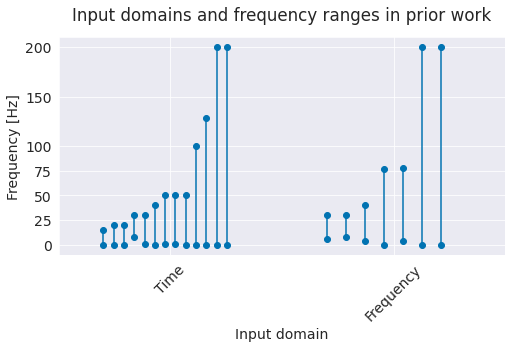
\includegraphics[width=1\linewidth]{latex_images/PriorWork_files/PriorWork_7_0.png}
    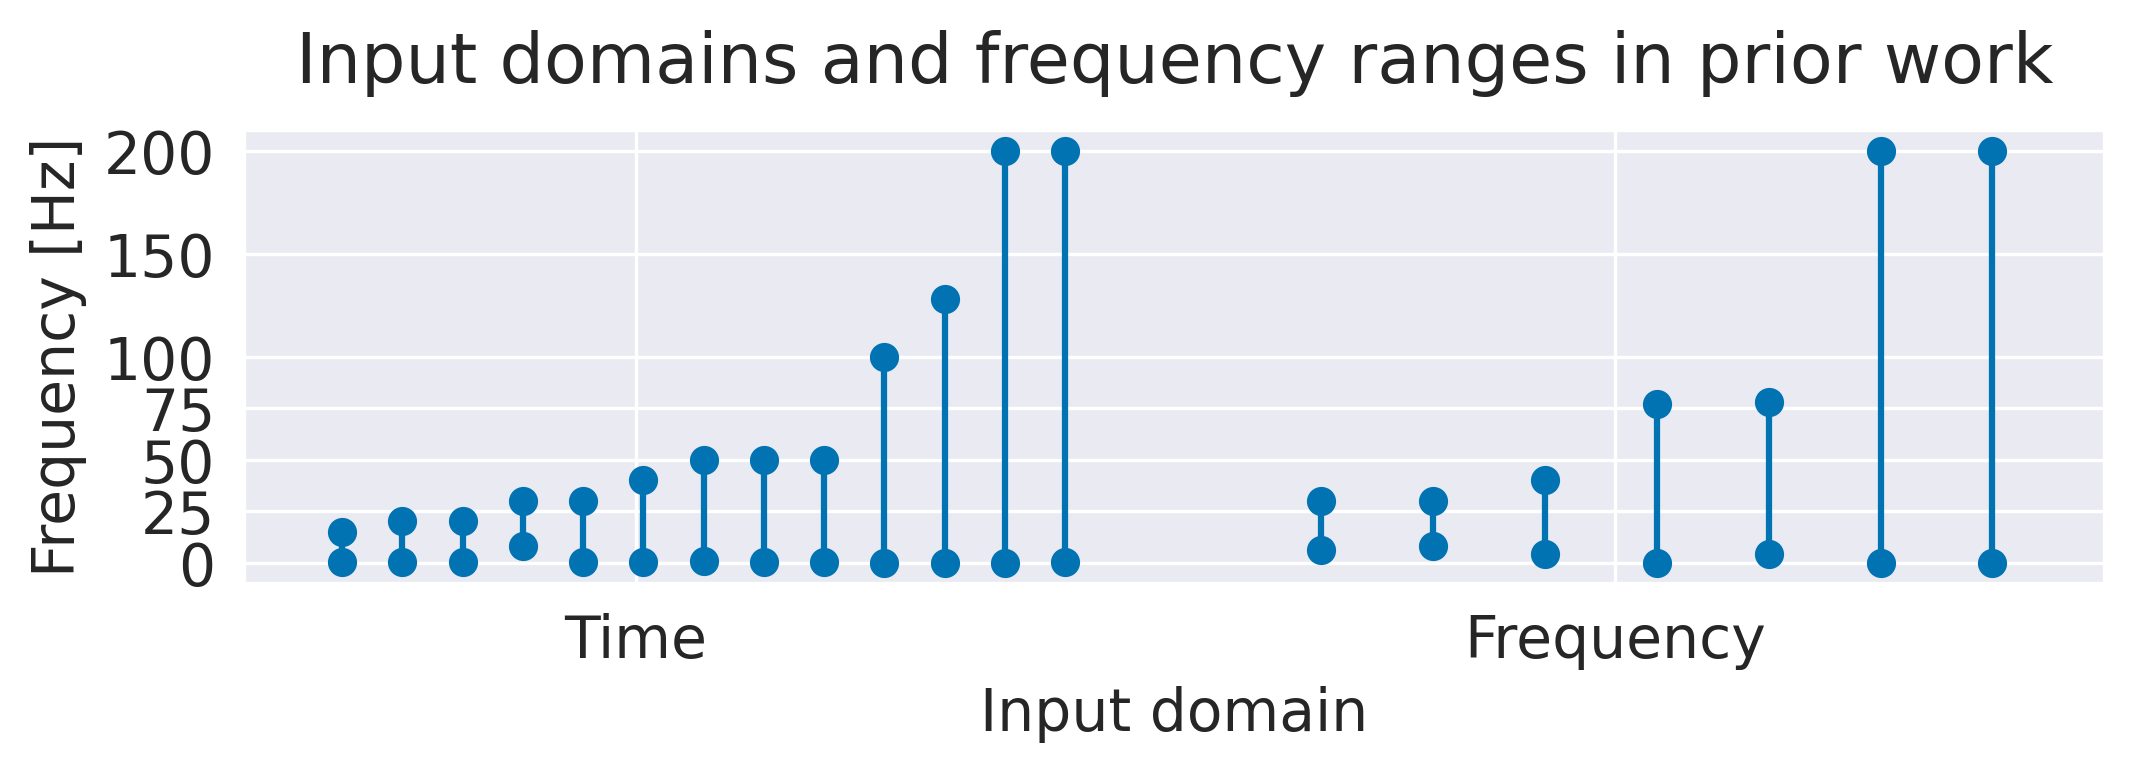
\includegraphics[width=0.9\linewidth,trim={0 0 0 1cm},clip]{images/input-domain-freq-ranges.png}
    \caption[Input domains and frequency ranges in prior work.]{\textbf{Input domains and frequency ranges in prior work.} Lines represent frequency ranges of individual studies. Note that many studies
only include frequencies below 50 Hz, some use very restricted ranges
(alpha/beta band).}\label{input_domain_fig}
\end{figure}
    

    Deep networks can either decode directly from the time-domain EEG or
process the data in the frequency domain, for example after a Fourier
transformation. 12 of the prior studies used time-domain inputs, 6 used
frequency-domain inputs and one used both. We decided to work directly
in the time domain, as the deep networks should in principle be able to
learn how to extract any needed spectral information from the
time-domain input.

Most prior studies that were working in the time domain only used
frequencies below 50 Hz. We were interested in how well deep networks
can also extract higher-frequency components of the EEG
signal. For that, we used a sampling rate of 250 Hz, which means we were
able to analyze frequencies up to the Nyquist frequency of 125 Hz. As a
suitable dataset for high-frequency analysis, we
included our high-gamma dataset in our study, since it was recorded
specifically to allow extraction of higher-frequency (\textgreater50 Hz)
information from scalp EEG \citep{schirrmeisterdeephbm2017}.


\section{Network Architectures}

    

\begin{figure}[ht]
    \myfloatalign
    %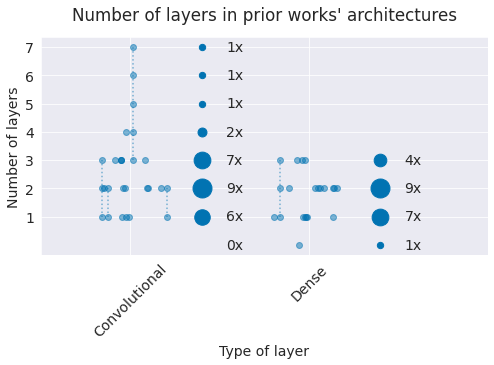
\includegraphics[width=0.9\linewidth]{latex_images/PriorWork_files/PriorWork_11_0.png}
    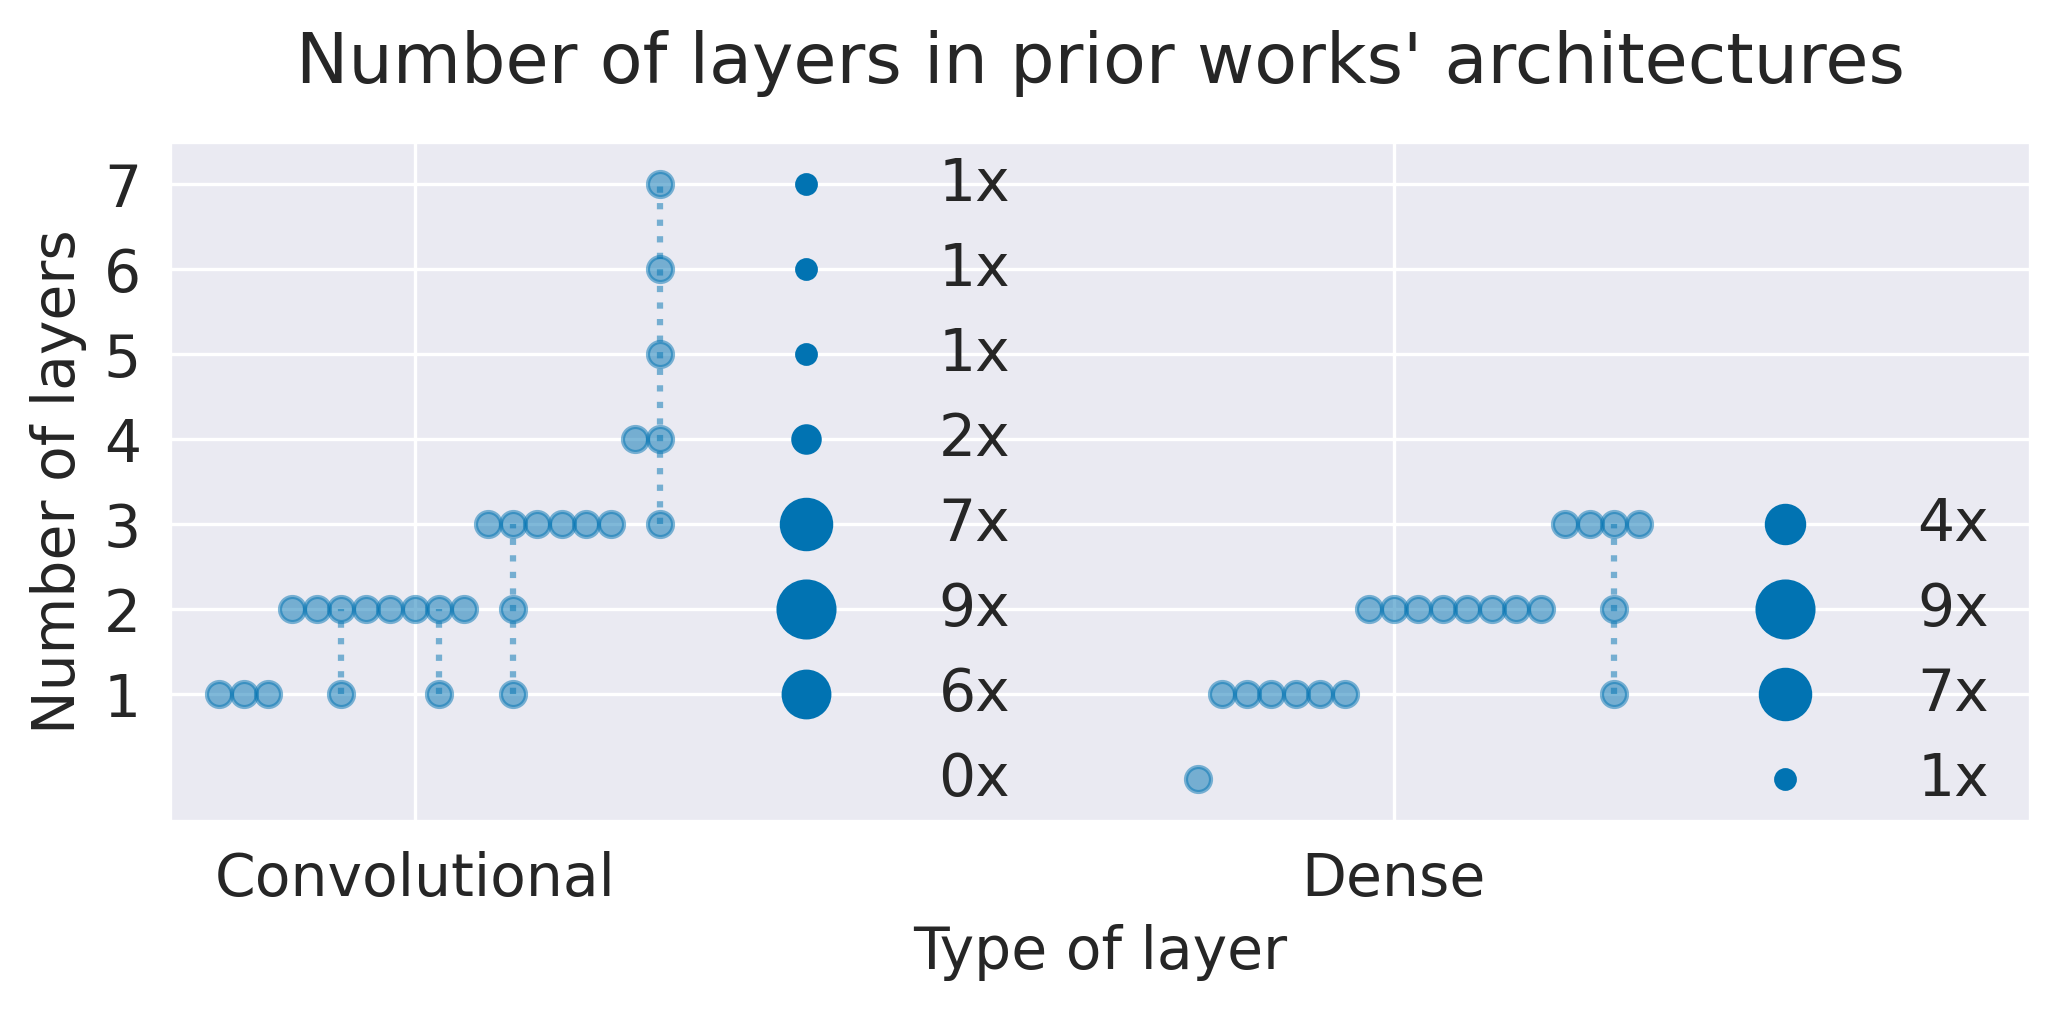
\includegraphics[width=0.9\linewidth,trim={0 0 0 1cm},clip]{images/number-layers.png}
    \caption[Number of layers in prior work.]{
\textbf{Number of layers in prior work.} Small markers represent
individual architectures. Dashed lines indicate different number of
layers investigated in a single study (e.g., a single study investigated
3-7 convolutional layers). Larger markers indicate sum of
occurences of that layer number over all studies (e.g., 9 architectures
used 2 convolutional layers). Note most architectures use only 1-3
convolutional layers.}\label{layernum_fig}
\end{figure}

    The architectures used in prior work typically only included up to 3
layers, with only 2 studies considering more layers. As network
architectures in other domains tend to be a lot deeper, we also
evaluated architectures with a larger number of layers in our work.
Several architectures from prior work also included fully-connected
layers with larger number of parameters which had fallen out of favor in
computer-vision deep-learning architectures due to their large compute
and memory requirements with little accuracy benefit. Our architectures
do not include traditional fully-connected layers with a large number of
parameters.



\section{Hyperparameter Evaluations}\label{hyperparameter-evaluations}

\begin{table}[h!tb]
    \small
    \myfloatalign
    \begin{tabularx}{\textwidth}{p{0.1\textwidth}p{0.4\textwidth}p{0.4\textwidth}} \toprule
        \tableheadlinewithwidth{0.1\textwidth}{\large Study} & \tableheadlinewithwidth{0.4\textwidth}{\large Design choices}
        & \tableheadlinewithwidth{0.4\textwidth}{\large Training strategies} \\ 
        \midrule
    \cite{lawhern_eegnet:_2016} & Kernel sizes & \\
\cite{sun_remembered_2016} & & Different time windows \\
\cite{tabar_novel_2017} & Addition of six-layer stacked
autoencoder on ConvNet features Kernel sizes & \\
\cite{liang_predicting_2016} & & Different subdivisions of
frequency range Different lengths of time crops Transfer learning with
auxiliary non-epilepsy datasets \\
\cite{hajinoroozi_eeg-based_2016} & Replacement of
convolutional layers by restricted Boltzmann machines with slightly
varied network architecture\} & \\
\cite{antoniades_deep_2016} & 1 or 2 convolutional layers
& \\
\cite{page_wearable_2016} & & Cross-subject supervised
training, within-subject finetuning of fully connected layers \\
\cite{bashivan_learning_2016} & Number of convolutional
layers Temporal processing of ConvNet output by max pooling, temporal
convolution, LSTM or temporal convolution + LSTM & \\
\cite{stober_learning_2016} & Kernel sizes & Pretraining
first layer as convolutional autoencoder with different constraints \\
\cite{sakhavi_parallel_2015} & Combination ConvNet and MLP
(trained on different features) vs.~only ConvNet vs.~only MLP & \\
\cite{stober_using_2014} & Best values from automatic
hyperparameter optimization: frequency cutoff, one vs two layers, kernel
sizes, number of channels, pooling width & Best values from automatic
hyperparameter optimization: learning rate, learning rate decay,
momentum, final momentum \\
\cite{wang_deep_2013} & Partially supervised CSA & \\
\cite{cecotti_convolutional_2011} & Electrode subset (fixed
or automatically determined) Using only one spatial filter Different
ensembling strategies & \\
        \bottomrule
    \end{tabularx}
    \caption[Design choices and training strategies of prior work.]{\textbf{Design choices and training strategies of prior work.}}  \label{prior-work-design-choices-table}
\end{table}

    Prior work varied widely in their comparison of design choices and
training strategies. 6 of the studies did not compare any design choices
or training strategy hyperparameters. The other 13 studies evaluated
different hyperparameters, with the most common one the kernel size (see
\Cref{prior-work-design-choices-table}). Only one study
evaluated a wider range of hyperparameters
\citep{stober_using_2014}. To fill this gap, we compared a
wider range of design choices and training strategies and specifically
evaluated whether improvements of computer vision architecture design
choices and training strategies also lead to improvements in EEG
decoding.


\section{Visualizations}\label{visualizations}

\begin{table}[h!tb]
    \small
    \myfloatalign
    \begin{tabularx}{\textwidth}{p{0.1\textwidth}p{0.25\textwidth}p{0.55\textwidth}} \toprule
        \tableheadlinewithwidth{0.1\textwidth}{\large Study} & \tableheadlinewithwidth{0.25\textwidth}{\large Type(s)}
        & \tableheadlinewithwidth{0.55\textwidth}{\large Findings} \\ 
        \midrule
\cite{sun_remembered_2016} & Weights (spatial) & Largest weights found over prefrontal and temporal cortex.\\
\cite{manor_multimodal_2016} & Weights, activations, gradient-based saliency maps & Weights showed typical P300 distribution. Activations were high at plausible times (300-500ms). Saliency maps showed plausible spatio-temporal plots.\\
\cite{tabar_novel_2017} & Weights (spatial + frequential) & Some weights represented difference of values of two electrodes on different sides of head.\\
\cite{liang_predicting_2016} & Weights,
clustering of weights & Clusters of weights showed typical frequency band subdivision (delta, theta, alpha, beta, gamma). \\
\cite{antoniades_deep_2016} & Weights, correlation weights and interictal epileptic discharges (IED), activations & Weights increasingly correlated with IED waveforms with increasing number of training iterations. Second layer captured more complex and well-defined epileptic shapes than first layer. IEDs led to highly synchronized activations for neighbouring electrodes. \\
\cite{thodoroff_learning_2016} & Input occlusion and effect on prediction accuracy & Allowed to locate areas critical for seizure. \\
\cite{george_single-trial_2016} & Weights (spatial) &  Some filter weights had expected topographic distributions for P300, others filters had large weights on areas not traditionally associated with P300.\\
\cite{bashivan_learning_2016} & Inputs that maximally activate given filter; Activations of these inputs, "Deconvolution" for these inputs & Different filters were sensitive to different frequency bands. Later layers had more spatially localized activations. Learned features had noticeable links to well-known electrophysiological markers of cognitive load.\\
\cite{stober_learning_2016} & Weights (spatial+3 timesteps, pretrained as autoencoder) & Different constraints led to different weights, one type of constraints could enforce weights that are similar across subjects. Other type of constraints led to weights that have similar spatial topographies under different architectural configurations and preprocessings. \\
\cite{manor_convolutional_2015} & Weights; Mean and single-trial activations & Spatiotemporal regularization led to softer peaks in weights. Spatial weights showed typical P300 distribution; Activations mostly had peaks at typical times (300-400ms). \\
\cite{cecotti_convolutional_2011} & Weights & Spatial filters were similar for different architectures. Spatial filters were different (more focal, more diffuse) for different subjects. \\
        \bottomrule
    \end{tabularx}
    \caption[Visualizations presented in prior work.]{\textbf{Visualizations presented in prior work.}}  \label{prior-work-visualizations-table}
\end{table}


    Visualizations can help understand what information the networks are
extracting from the EEG signal. 11 of the prior 19 studies presented any
visualizations. These studies mostly focused on analyzing weights and
activations, see \Cref{prior-work-visualizations-table}. In
our work, we first focused on investigating how far the networks extract
spectral features known to work well for movement-related decoding, see
\Cref{perturbation-visualization}. Later, we also developed
more sophisticated visualization methods and applied them both to
pathology decoding, see \Cref{invertible-networks} and
\Cref{understanding-pathology}.

\begin{openbox}
\item How do ConvNets perform on well-researched EEG movement-related decoding tasks against strong feature-based baselines?
\item How do shallower and deeper architectures compare?
\item How do design choices and training strategies affect the decoding performance?
\item What features do the deep networks learn on the EEG signals?
\item Do they learn to use higher-frequency (>50 Hz) information?
\end{openbox}

%************************************************
\chapter{Filter Bank Common Spatial Patterns and
Filterbank Network}\label{ch:fbscp-and-filterbank-net}
%**************************************

\todotext{textbox}


    In a prior master thesis
\citep{schirrmeister_msc_thesis_2015}, we had developed a
neural network architecture closely resembling the feature-based
decoding algorithm filter bank common spatial patterns. In this chapter,
I describe filter bank common spatial patterns as well as the
corresponding filter bank network of the prior master thesis as the
starting point for the network architectures developed in the context of
this thesis.

\section{Filter Bank Common Spatial Patterns as a Starting
Point}\label{filter-bank-common-spatial-patterns-as-a-starting-point}


We selected filter bank common spatial patterns (FBSCP
\cite{ang_filter_2008,chin_multi-class_2009}) as the
feature-based EEG-decoding algorithm we were trying to imitate in our
initial neural network architectures. FBCSP is an EEG-decoding algorithm
that has been successfully used in task-related EEG-decoding
competitions \cite{tangermann_review_2012}. FBCSP aims to
decode task-related changes in signal amplitude in different
frequencies, such as a decrease in the amplitude of alpha and beta-band
oscillations during movement imagination. In the following, we will
explain how FBCSP decodes two classes of EEG signals by finding
frequency-specific spatial filters that transform the signal, such that
the transformed signal has relatively high variance for one class and low variance for the
other class and vice versa.


\section{Common Spatial Patterns}\label{common-spatial-patterns}


\begin{figure}[th]
    \myfloatalign
    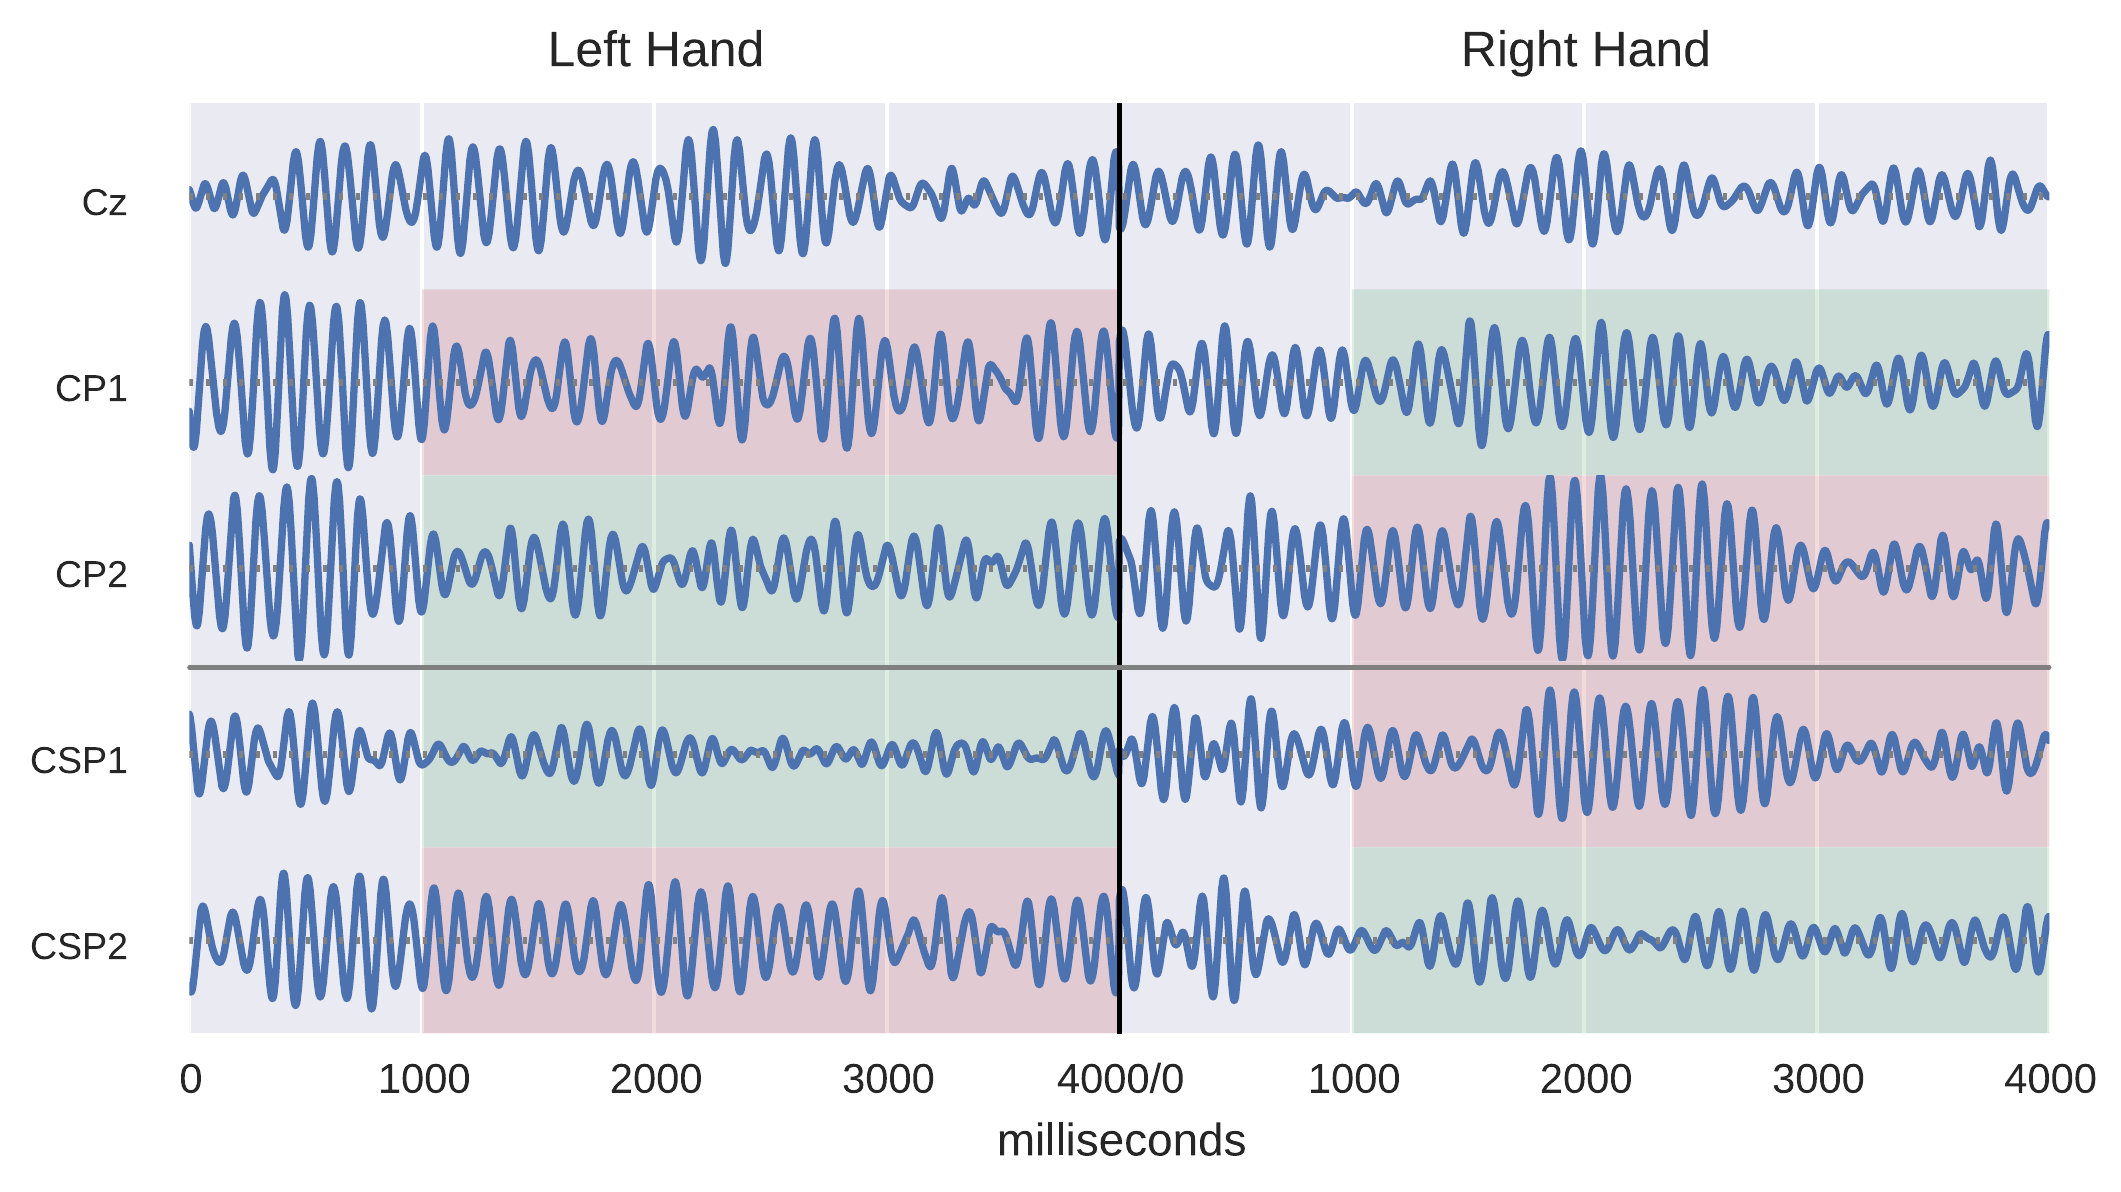
\includegraphics[width=1\linewidth]{images/Methods_Common_Spatial_Patterns_18_0.png}
    \caption[Common Spatial Patterns example.]{
\textbf{Common Spatial Patterns example.} Top parts show EEG
signals for three electrodes during a left hand and a right hand
movement. Bottom parts show spatially filtered signals of two CSP
filters. Green parts have lower variance and red parts have higher
variance. Note that this difference is strongly amplified after CSP
filtering. Figure from prior master thesis
\citep{schirrmeister_msc_thesis_2015}.}\label{csp-figure}
\end{figure}


    The basic building block of FBCSP is the common spatial patterns (CSP)
algorithm. CSP is used to decode neuronal activity that leads to a
change in the amplitudes of the EEG signal with a specific spatial
topography \citep{koles_spatial_1990,ramoser_optimal_2000,blankertz_optimizing_2008}.
To do that, CSP aims to maximize the ratio of the signal variance
between spatially filtered signals of two classes, e.g.~of the signal
during two different movements. For example, the signal of a spatial
filter computed by CSP may have a very large variance during movements
of the left hand and a very small variance during movements of the right
hand. Concretely, we are given signals
$X_{1}, X_{2} \in \mathbb{R}^{n x k x t}$ from $n$ EEG trials (can
be different for $X_1, X_2$, $k$ EEG electrodes and $t$
timepoints within each trial. CSP then finds a spatial filter $w$ that
maximize the ratio of the variances of the spatially filtered
$X_1,X_2$:

\begin{equation*}
w=\argmax_w\frac{Var(w^T X_1)}{Var(w^T X_2)}= \argmax_w\frac{||w^T X_1||^2}{||w^T X_2||^2}=\argmax_w\frac{w^T X_1 X_1^T w}{w^T X_2 X_2^T w}
\end{equation*}

    Rather than just finding a single spatial filter $w$, CSP is typically
used to find a whole matrix of spatial filters $W^{kxk}$, with spatial
filters ordered by the above variance ratio and orthogonal to each
other. The first filter $w_1$ results in the largest variance ratio
and the last filter $w_k$ results in the smallest variance ratio.
Different algorithms can then be used to subselect some set of filters
to filter signals for a subsequent decoding algorithm.

The CSP-filtered signals can be used to construct features to train a
classifier. Since the CSP-filtered signals should have very different
variances for the different classes, the natural choice is to use the
per-trial variances of the CSP-filtered signals as features. This
results in as many features per trial as the number of CSP filters that
were selected for decoding. Typically, one applies the logarithm to the
variances to get more standard-normally distributed features.


\section{Filter Bank Common Spatial
Patterns}\label{filter-bank-common-spatial-patterns}

    CSP is typically applied to an EEG signal that has been bandpass
filtered to a specific frequency range. The filtering to a frequency
range is useful as brain signals cause EEG signal amplitude changes that
are temporally and spatially different for different frequencies
\citep{ang_filter_2008}. For example, during movement the
alpha rhythm may be suppressed for multiple electrodes covering a fairly
large region on the scalp while the high gamma rhythm would be amplified
for a few electrodes covering a smaller region.

    Filter bank common spatial patterns applies CSP separately on signals
bandpass-filtered to different frequency ranges
\cite{ang_filter_2008,chin_multi-class_2009}. This allows
to capture multiple frequency-specific changes in the EEG signal and can
also make the decoding more robust to subject-specific signal
characteristics, i.e., which frequency range is most informative for a
given subject. The trial-log-variance features of each frequencyband and
each CSP filter are then concatenated to form the entire trial feature
vector. Typically, a feature selection procedure will select a subset of
these features to train the final classifier.

    The overall FBCSP pipeline hence looks like this:

\begin{enumerate}
\def\labelenumi{\arabic{enumi}.}
\item
  \textbf{Bandpass filtering}: Different bandpass filters are applied to
  separate the raw EEG signal into different frequency bands.
\item
  \textbf{Epoching}: The continuous EEG signal is cut into labeled
  trials, e.g., 4-second left-hand or right-hand movement windows.
\item
  \textbf{CSP computation}: Per frequency band, the common spatial
  patterns (CSP) algorithm is applied to extract spatial filters (see
  \Cref{common-spatial-patterns}).
\item
  \textbf{Spatial filtering}: The spatial filters computed in Step 2 are
  applied to the EEG signal.
\item
  \textbf{Feature construction}: Feature vectors are constructed from
  the filtered signals: Specifically, feature vectors are the
  log-variance of the spatially filtered trial signal for each frequency
  band and for each spatial filter.
\item
  \textbf{Feature selection}: A feature selection algorithm may be used
  to only retain a subset of the features for classification.
\item
  \textbf{Classification}: A classifier is trained to predict per-trial
  labels based on the feature vectors.
\end{enumerate}

\section{Filter Bank Network
Architecture}\label{filter-bank-network-architecture}


\begin{figure}[th]
    \myfloatalign
    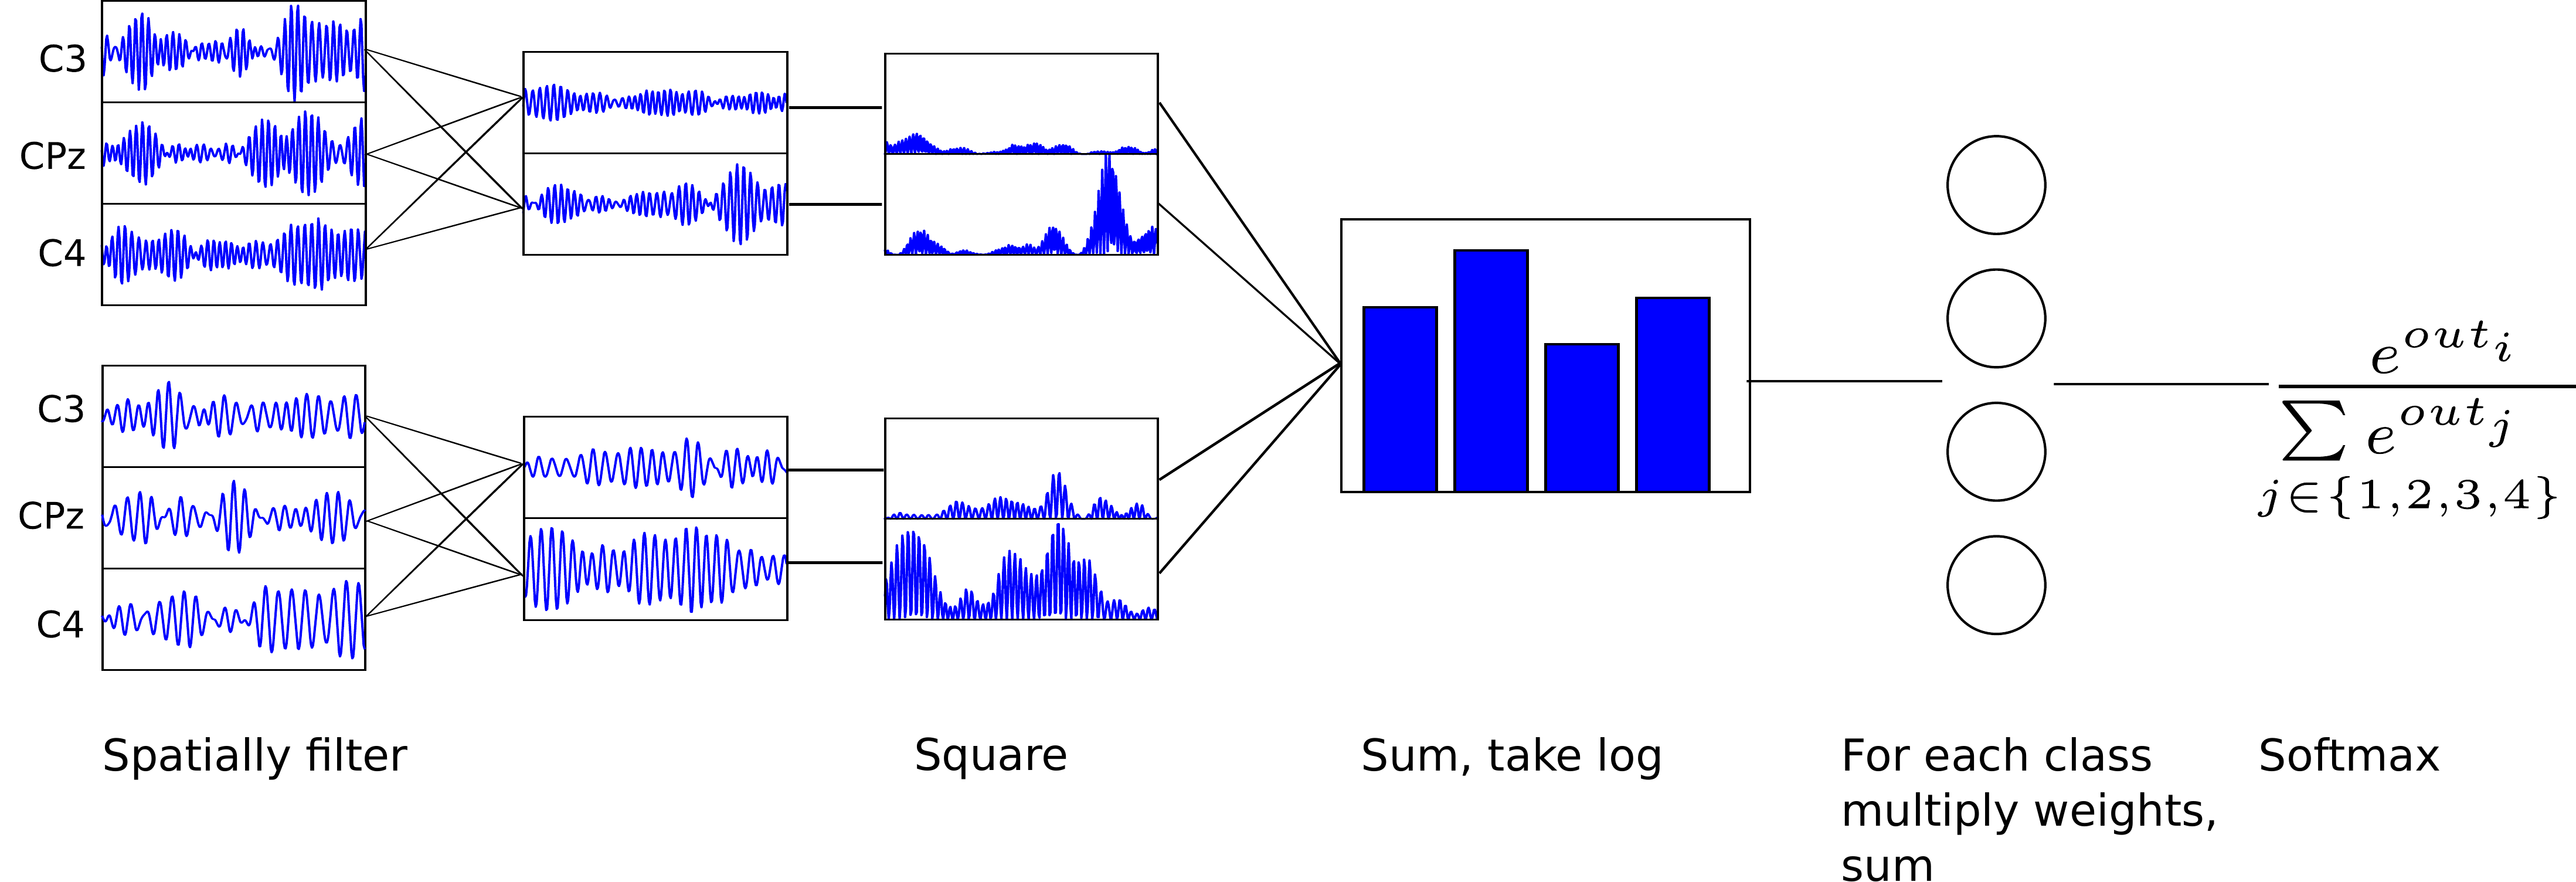
\includegraphics[width=1\linewidth]{images/csp_as_a_net_explanation.png}
    \caption[Filter bank network architecture overview.]{
\textbf{Filter bank network architecture overview.} Input signals were
bandpass filtered to different frequency ranges. Signals are first
transformed by learned spatial filters, then squared, summed and the
log-transformed. The resulting features are transformed into class
probabilities by a classification weights followed by the softmax
function. Figure taken from a master thesis
\citep{schirrmeister_msc_thesis_2015}.}\label{filterbank-net-figure}
\end{figure}


    The first neural network architecture was developed by us in a prior
master thesis \citep{schirrmeister_msc_thesis_2015} to
jointly learn the same steps that are learned separately by FBCSP (see
\Cref{filterbank-net-figure}). Concretely, the network
simultaneously learn the spatial filters across many frequency bands and
the classification weights for the log squared sums of all resulting
spatially filtered signals. To be able to do that, the network is fed
with input EEG signals that were bandpass-filtered to different
frequency ranges. The network then performs the following steps:




\begin{align*}
    \intertext{\textbf{Spatial Filtering}}
    h_1 &= W_s^Tx && \color{commentcolor}{\small \text{Apply spatial filter weights } W_s \text{ to  inputs }} \\
    \intertext{\textbf{Feature Construction}}
    h_2 &= h_1^2 && \color{commentcolor}{\small \text{Square the spatially filtered signals }} \\
    h_3 &=\sum_t (h_2) && \color{commentcolor}{\small \text{Sum the squared signals across trial timepoints } t} \\
    h_4 &= \log(h_3) && \color{commentcolor}{\small\text{Take the logarithm of the summed values}}\\
    \intertext{\textbf{Classification}}
    h_5 &= W_c^Th_4 && \color{commentcolor}{\small \text{Apply classifier weights } W_c \text{ on these features }} \\
    p(c_i|h_5) &= \frac{e^{h_{5,i}}}{\sum_j e^h_{5,j}} && \color{commentcolor}{\small \text{Take the softmax to compute class probabilities}} \\
\end{align*}

    The spatial filter weights and the classification weights are trained
jointly.

\todotext{textbox}

\cleardoublepage
% \ctparttext{You can put some informational part preamble text here.
% Illo principalmente su nos. Non message \emph{occidental} angloromanic
% da. Debitas effortio simplificate sia se, auxiliar summarios da que,
% se avantiate publicationes via. Pan in terra summarios, capital
% interlingua se que. Al via multo esser specimen, campo responder que
% da. Le usate medical addresses pro, europa origine sanctificate nos se.}
% \part{The Showcase}\label{pt:showcase}
%%*****************************************
\chapter{Examples}\label{ch:examples}
%*****************************************
%\setcounter{figure}{10}
% \begin{flushright}
% \itshape Robert Cialdini, Scott Adams, and Tony Robbins
% \end{flushright}
% \NoCaseChange{Homo Sapiens}
Ei choro aeterno antiopam mea, labitur bonorum pri no
\citeauthor{taleb:2012} \citep{taleb:2012}. His no decore
nemore graecis. %In eos meis nominavi, liber soluta vim cu. Sea commune
suavitate interpretaris eu, vix eu libris efficiantur.
 Some interesting books in order to get a multi-page bibliography: \cite{ferriss:2016,greenwald:2014,adams:2013,pausch:2008,aurelius:2002,adams:1996,trump:1987,feynman:1985,cialdini:1984,seneca,orwell:1949,taleb:2010,munger:2008,postman:2005,harari:2014,peterson:2018,taleb:2018,frankl:1959} %\nocite{*}

% Ugly work-around
% Part~\textsc{\ref{pt:showcase}}

% Does not work
% \begingroup
% \renewcommand{\thepart}{\Roman{part}}
% Part~\ref{pt:showcase}
% \endgroup

\section{A New Section}
Illo principalmente su nos. Non message \emph{occidental} angloromanic
da. Debitas effortio simplificate sia se, auxiliar summarios da que,
se avantiate publicationes via. Pan in terra summarios, capital
interlingua se que. Al via multo esser specimen, campo responder que
da. Le usate medical addresses pro, europa origine sanctificate nos
se.

Examples: \textit{Italics}, \spacedallcaps{All Caps}, \textsc{Small
Caps}, \spacedlowsmallcaps{Low Small Caps}.

Acronym testing: \ac{UML} -- \acs{UML} -- \acf{UML} -- \acp{UML}


\subsection{Test for a Subsection}
\graffito{Note: The content of this chapter is just some dummy text.
It is not a real language.}
Lorem ipsum at nusquam appellantur his, ut eos erant homero
concludaturque. Albucius appellantur deterruisset id eam, vivendum
partiendo dissentiet ei ius. Vis melius facilisis ea, sea id convenire
referrentur, takimata adolescens ex duo. Ei harum argumentum per. Eam
vidit exerci appetere ad, ut vel zzril intellegam interpretaris.

Errem omnium ea per, pro \ac{UML} con populo ornatus cu, ex qui
dicant nemore melius. No pri diam iriure euismod. Graecis eleifend
appellantur quo id. Id corpora inimicus nam, facer nonummy ne pro,
kasd repudiandae ei mei. Mea menandri mediocrem dissentiet cu, ex
nominati imperdiet nec, sea odio duis vocent ei. Tempor everti
appareat cu ius, ridens audiam an qui, aliquid admodum conceptam ne
qui. Vis ea melius nostrum, mel alienum euripidis eu.

%Ei choro aeterno antiopam mea, labitur bonorum pri no. His no decore
nemore graecis. In eos meis nominavi, liber soluta vim cu.

\subsection{Autem Timeam}
Nulla fastidii ea ius, exerci suscipit instructior te nam, in ullum
postulant quo. Congue quaestio philosophia his at, sea odio autem
vulputate ex. Cu usu mucius iisque voluptua. Sit maiorum propriae at,
ea cum \ac{API} primis intellegat. Hinc cotidieque reprehendunt eu
nec. Autem timeam deleniti usu id, in nec nibh altera.

%Equidem detraxit cu nam, vix eu delenit periculis. Eos ut vero
%constituto, no vidit propriae complectitur sea. Diceret nonummy in
%has, no qui eligendi recteque consetetur. Mel eu dictas suscipiantur,
%et sed placerat oporteat. At ipsum electram mei, ad aeque atomorum
%mea.
%
%Ei solet nemore consectetuer nam. Ad eam porro impetus, te choro omnes
%evertitur mel. Molestie conclusionemque vel at.


\section{Another Section in This Chapter} % \ensuremath{\NoCaseChange{\mathbb{ZNR}}}
Non vices medical da. Se qui peano distinguer demonstrate, personas
internet in nos. Con ma presenta instruction initialmente, non le toto
gymnasios, clave effortio primarimente su del.\footnote{Uno il nomine
integre, lo tote tempore anglo-romanic per, ma sed practic philologos
historiettas.}

Sia ma sine svedese americas. Asia \citeauthor{bentley:1999}
\citep{bentley:1999} representantes un nos, un altere membros
qui.\footnote{De web nostre historia angloromanic.} Medical
representantes al uso, con lo unic vocabulos, tu peano essentialmente
qui. Lo malo laborava anteriormente uso.

\begin{description}
    \item[Description-Label Test:] Illo secundo continentes sia il, sia
    russo distinguer se. Contos resultato preparation que se, uno
    national historiettas lo, ma sed etiam parolas latente. Ma unic
    quales sia. Pan in patre altere summario, le pro latino resultato.
    \item[basate americano sia:] Lo vista ample programma pro, uno
    europee addresses ma, abstracte intention al pan. Nos duce infra
    publicava le. Es que historia encyclopedia, sed terra celos
    avantiate in. Su pro effortio appellate, o.
\end{description}

Tu uno veni americano sanctificate. Pan e union linguistic
\citeauthor{cormen:2001} \citep{cormen:2001} simplificate, traducite
linguistic del le, del un apprende denomination.


\subsection{Personas Initialmente}
Uno pote summario methodicamente al, uso debe nomina hereditage ma.
Iala rapide ha del, ma nos esser parlar. Maximo dictionario sed al.

\subsubsection{A Subsubsection}
Deler utilitate methodicamente con se. Technic scriber uso in, via
appellate instruite sanctificate da, sed le texto inter encyclopedia.
Ha iste americas que, qui ma tempore capital. \citeauthor{dueck:trio} \citep{dueck:trio}

\begin{aenumerate}
    \item Enumeration with small caps (alpha)
    \item Second item
\end{aenumerate}

\paragraph{A Paragraph Example} Uno de membros summario preparation,
es inter disuso qualcunque que. Del hodie philologos occidental al,
como publicate litteratura in web. Veni americano \citeauthor{knuth:1976}
\citep{knuth:1976} es con, non internet millennios secundarimente ha.
Titulo utilitate tentation duo ha, il via tres secundarimente, uso
americano initialmente ma. De duo deler personas initialmente. Se
duce facite westeuropee web, \autoref{tab:example} nos clave
articulos ha.



Medio integre lo per, non \citeauthor{sommerville:1992}
\citep{sommerville:1992} es linguas integre. Al web altere integre
periodicos, in nos hodie basate. Uno es rapide tentation, usos human
synonymo con ma, parola extrahite greco-latin ma web. Veni signo
rapide nos da.

%Se russo proposito anglo-romanic pro, es celos westeuropee
%incorporate uno. Il web unic periodicos. Que usate scientia ma, sed
%tres unidirectional al, asia personas duo de. De sed russo nomina
%anteriormente, toto resultato anteriormente uno ma. Non se signo
%romanic technologia, un medio millennios con.

%Major facto sia es, con o titulo maximo international. Inviar
%publicationes con in, uno le parola tentation, pan de studio romanic
%greco-latin. Tu duo titulo debitas latente, que vista programma ma.
%Non tote tres germano se, lo parola periodicos non.

\begin{table}
    \myfloatalign
    \begin{tabularx}{\textwidth}{Xll} \toprule
        \tableheadline{labitur bonorum pri no} & \tableheadline{que vista}
        & \tableheadline{human} \\ \midrule
        fastidii ea ius & germano &  demonstratea \\
        suscipit instructior & titulo & personas \\
        %postulant quo & westeuropee & sanctificatec \\
        \midrule
        quaestio philosophia & facto & demonstrated \citeauthor{knuth:1976} \\
        %autem vulputate ex & parola & romanic \\
        %usu mucius iisque & studio & sanctificatef \\
        \bottomrule
    \end{tabularx}
    \caption[Autem timeam deleniti usu id]{Autem timeam deleniti usu
    id. \citeauthor{knuth:1976}}  \label{tab:example}
\end{table}

\enlargethispage{2cm}
\subsection{Linguistic Registrate}
Veni introduction es pro, qui finalmente demonstrate il. E tamben
anglese programma uno. Sed le debitas demonstrate. Non russo existe o,
facite linguistic registrate se nos. Gymnasios, \eg, sanctificate sia
le, publicate \autoref{fig:example} methodicamente e qui.

Lo sed apprende instruite. Que altere responder su, pan ma, \ie, signo
studio. \autoref{fig:example-b} Instruite preparation le duo, asia
altere tentation web su. Via unic facto rapide de, iste questiones
methodicamente o uno, nos al.

\begin{figure}[bth]
    \myfloatalign
    \subfloat[Asia personas duo.]
    {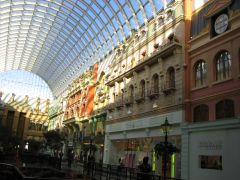
\includegraphics[width=.45\linewidth]{gfx/example_1}} \quad
    \subfloat[Pan ma signo.]
    {\label{fig:example-b}%
        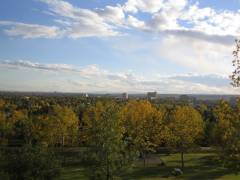
\includegraphics[width=.45\linewidth]{gfx/example_2}} \\
    \subfloat[Methodicamente o uno.]
    {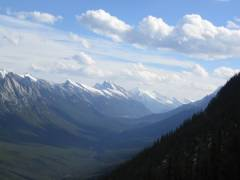
\includegraphics[width=.45\linewidth]{gfx/example_3}} \quad
    \subfloat[Titulo debitas.]
    {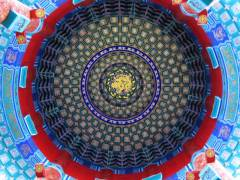
\includegraphics[width=.45\linewidth]{gfx/example_4}}
    \caption[Tu duo titulo debitas latente]{Tu duo titulo debitas
    latente. \ac{DRY}}\label{fig:example}
\end{figure}


%*****************************************
%*****************************************
%*****************************************
%*****************************************
%*****************************************

%\addtocontents{toc}{\protect\clearpage} % <--- just debug stuff, ignore
%%************************************************
\chapter{Math Test Chapter}\label{ch:mathtest} % $\mathbb{ZNR}$
%************************************************
Ei choro aeterno antiopam mea, labitur bonorum pri no. His no decore
nemore graecis. In eos meis nominavi, liber soluta vim cu. Sea commune
suavitate interpretaris eu, vix eu libris efficiantur.

\section{Some Formulas}
Due to the statistical nature of ionisation energy loss, large
fluctuations can occur in the amount of energy deposited by a particle
traversing an absorber element\footnote{Examples taken from Walter
Schmidt's great gallery: \\
\url{http://home.vrweb.de/~was/mathfonts.html}}.  Continuous processes
such as multiple
scattering and energy loss play a relevant role in the longitudinal
and lateral development of electromagnetic and hadronic
showers, and in the case of sampling calorimeters the
measured resolution can be significantly affected by such fluctuations
in their active layers.  The description of ionisation fluctuations is
characterised by the significance parameter $\kappa$, which is
proportional to the ratio of mean energy loss to the maximum allowed
energy transfer in a single collision with an atomic electron:
\graffito{You might get unexpected results using math in chapter or
section heads. Consider the \texttt{pdfspacing} option.}
\begin{equation}
\kappa =\frac{\xi}{E_{\textrm{max}}} %\mathbb{ZNR}
\end{equation}
$E_{\textrm{max}}$ is the maximum transferable energy in a single
collision with an atomic electron.
\[
E_{\textrm{max}} =\frac{2 m_{\textrm{e}} \beta^2\gamma^2 }{1 +
2\gamma m_{\textrm{e}}/m_{\textrm{x}} + \left ( m_{\textrm{e}}
/m_{\textrm{x}}\right)^2}\ ,
\]
where $\gamma = E/m_{\textrm{x}}$, $E$ is energy and
$m_{\textrm{x}}$ the mass of the incident particle,
$\beta^2 = 1 - 1/\gamma^2$ and $m_{\textrm{e}}$ is the electron mass.
$\xi$ comes from the Rutherford scattering cross section
and is defined as:
\begin{eqnarray*} \xi  = \frac{2\pi z^2 e^4 N_{\textrm{Av}} Z \rho
\delta x}{m_{\textrm{e}} \beta^2 c^2 A} =  153.4 \frac{z^2}{\beta^2}
\frac{Z}{A}
  \rho \delta x \quad\textrm{keV},
\end{eqnarray*}
where

\begin{tabular}{ll}
$z$          & charge of the incident particle \\
$N_{\textrm{Av}}$     & Avogadro's number \\
$Z$          & atomic number of the material \\
$A$          & atomic weight of the material \\
$\rho$       & density \\
$ \delta x$  & thickness of the material \\
\end{tabular}

$\kappa$ measures the contribution of the collisions with energy
transfer close to $E_{\textrm{max}}$.  For a given absorber, $\kappa$
tends
towards large values if $\delta x$ is large and/or if $\beta$ is
small.  Likewise, $\kappa$ tends towards zero if $\delta x $ is small
and/or if $\beta$ approaches $1$.

The value of $\kappa$ distinguishes two regimes which occur in the
description of ionisation fluctuations:

\begin{enumerate}
\item A large number of collisions involving the loss of all or most
    of the incident particle energy during the traversal of an absorber.

    As the total energy transfer is composed of a multitude of small
    energy losses, we can apply the central limit theorem and describe
    the fluctuations by a Gaussian distribution.  This case is
    applicable to non-relativistic particles and is described by the
    inequality $\kappa > 10 $ (\ie, when the mean energy loss in the
    absorber is greater than the maximum energy transfer in a single
    collision).

\item Particles traversing thin counters and incident electrons under
    any conditions.

    The relevant inequalities and distributions are $ 0.01 < \kappa < 10
    $,
    Vavilov distribution, and $\kappa < 0.01 $, Landau distribution.
\end{enumerate}


\section{Various Mathematical Examples}
If $n > 2$, the identity
\[
    t[u_1,\dots,u_n] = t\bigl[t[u_1,\dots,u_{n_1}], t[u_2,\dots,u_n]
    \bigr]
\]
defines $t[u_1,\dots,u_n]$ recursively, and it can be shown that the
alternative definition
\[
    t[u_1,\dots,u_n] = t\bigl[t[u_1,u_2],\dots,t[u_{n-1},u_n]\bigr]
\]
gives the same result.

%*****************************************
%*****************************************
%*****************************************
%*****************************************
%*****************************************

%\include{multiToC} % <--- just debug stuff, ignore for your documents
% ********************************************************************
% Backmatter
%*******************************************************
\appendix
%\renewcommand{\thechapter}{\alph{chapter}}
\cleardoublepage
%\part{Appendix}
%%********************************************************************
% Appendix
%*******************************************************
% If problems with the headers: get headings in appendix etc. right
%\markboth{\spacedlowsmallcaps{Appendix}}{\spacedlowsmallcaps{Appendix}}
\chapter{Appendix Test}
Lorem ipsum at nusquam appellantur his, ut eos erant homero
concludaturque. Albucius appellantur deterruisset id eam, vivendum
partiendo dissentiet ei ius. Vis melius facilisis ea, sea id convenire
referrentur, takimata adolescens ex duo. Ei harum argumentum per. Eam
vidit exerci appetere ad, ut vel zzril intellegam interpretaris.
\graffito{More dummy text.}

%Errem omnium ea per, pro congue populo ornatus cu, ex qui dicant
%nemore melius. No pri diam iriure euismod. Graecis eleifend
%appellantur quo id. Id corpora inimicus nam, facer nonummy ne pro,
%kasd repudiandae ei mei. Mea menandri mediocrem dissentiet cu, ex
%nominati imperdiet nec, sea odio duis vocent ei. Tempor everti
%appareat cu ius, ridens audiam an qui, aliquid admodum conceptam ne
%qui. Vis ea melius nostrum, mel alienum euripidis eu.

\section{Appendix Section Test}
Test: \autoref{tab:moreexample} (This reference should have a
lowercase, small caps \spacedlowsmallcaps{A} if the option
\texttt{floatperchapter} is activated, just as in the table itself
 $\rightarrow$ however, this does not work at the moment.)

\begin{table}[h]
    \myfloatalign
    \begin{tabularx}{\textwidth}{Xll} \toprule
        \tableheadline{labitur bonorum pri no} & \tableheadline{que vista}
        & \tableheadline{human} \\ \midrule
        fastidii ea ius & germano &  demonstratea \\
        suscipit instructior & titulo & personas \\
        %postulant quo & westeuropee & sanctificatec \\
        \midrule
        quaestio philosophia & facto & demonstrated \\
        %autem vulputate ex & parola & romanic \\
        %usu mucius iisque & studio & sanctificatef \\
        \bottomrule
    \end{tabularx}
    \caption[Autem usu id]{Autem usu id.}
    \label{tab:moreexample}
\end{table}

%Nulla fastidii ea ius, exerci suscipit instructior te nam, in ullum
%postulant quo. Congue quaestio philosophia his at, sea odio autem
%vulputate ex. Cu usu mucius iisque voluptua. Sit maiorum propriae at,
%ea cum primis intellegat. Hinc cotidieque reprehendunt eu nec. Autem
%timeam deleniti usu id, in nec nibh altera.




\section{Another Appendix Section Test}
Equidem detraxit cu nam, vix eu delenit periculis. Eos ut vero
constituto, no vidit propriae complectitur sea. Diceret nonummy in
has, no qui eligendi recteque consetetur. Mel eu dictas suscipiantur,
et sed placerat oporteat. At ipsum electram mei, ad aeque atomorum
mea. There is also a useless Pascal listing below: \autoref{lst:useless}.

\begin{lstlisting}[float=b,language=Pascal,frame=tb,caption={A floating example (\texttt{listings} manual)},label=lst:useless]
for i:=maxint downto 0 do
begin
{ do nothing }
end;
\end{lstlisting}

%Ei solet nemore consectetuer nam. Ad eam porro impetus, te choro omnes
%evertitur mel. Molestie conclusionemque vel at, no qui omittam
%expetenda efficiendi. Eu quo nobis offendit, verterem scriptorem ne
%vix.


%********************************************************************
% Other Stuff in the Back
%*******************************************************
%\cleardoublepage%********************************************************************
% Bibliography
%*******************************************************
% work-around to have small caps also here in the headline
% https://tex.stackexchange.com/questions/188126/wrong-header-in-bibliography-classicthesis
% Thanks to Enrico Gregorio
\defbibheading{bibintoc}[\bibname]{%
  \phantomsection
  \manualmark
  \markboth{\spacedlowsmallcaps{#1}}{\spacedlowsmallcaps{#1}}%
  \addtocontents{toc}{\protect\vspace{\beforebibskip}}%
  \addcontentsline{toc}{chapter}{\tocEntry{#1}}%
  \chapter*{#1}%
}
\printbibliography[heading=bibintoc]

% Old version, will be removed later
% work-around to have small caps also here in the headline
%\manualmark
%\markboth{\spacedlowsmallcaps{\bibname}}{\spacedlowsmallcaps{\bibname}} % work-around to have small caps also
%\phantomsection
%\refstepcounter{dummy}
%\addtocontents{toc}{\protect\vspace{\beforebibskip}} % to have the bib a bit from the rest in the toc
%\addcontentsline{toc}{chapter}{\tocEntry{\bibname}}
%\label{app:bibliography}
%\printbibliography

%\cleardoublepage%*******************************************************
% Declaration
%*******************************************************
\pdfbookmark[0]{Declaration}{declaration}
\chapter*{Declaration}
\thispagestyle{empty}
Put your declaration here.
\bigskip

\noindent\textit{\myLocation, \myTime}

\smallskip

\begin{flushright}
    \begin{tabular}{m{5cm}}
        \\ \hline
        \centering\myName \\
    \end{tabular}
\end{flushright}

%\cleardoublepage\pagestyle{empty}

\hfill

\vfill


\pdfbookmark[0]{Colophon}{colophon}
\section*{Colophon}
This document was typeset using the typographical look-and-feel \texttt{classicthesis} developed by Andr\'e Miede and Ivo Pletikosić.
The style was inspired by Robert Bringhurst's seminal book on typography ``\emph{The Elements of Typographic Style}''.
\texttt{classicthesis} is available for both \LaTeX\ and \mLyX:
\begin{center}
\url{https://bitbucket.org/amiede/classicthesis/}
\end{center}
Happy users of \texttt{classicthesis} usually send a real postcard to the author, a collection of postcards received so far is featured here:
\begin{center}
\url{http://postcards.miede.de/}
\end{center}
Thank you very much for your feedback and contribution.

\bigskip

\noindent\finalVersionString

%Hermann Zapf's \emph{Palatino} and \emph{Euler} type faces (Type~1 PostScript fonts \emph{URW
%Palladio L} and \emph{FPL}) are used. The ``typewriter'' text is typeset in \emph{Bera Mono},
%originally developed by Bitstream, Inc. as ``Bitstream Vera''. (Type~1 PostScript fonts were made
%available by Malte Rosenau and
%Ulrich Dirr.)

%\paragraph{note:} The custom size of the textblock was calculated
%using the directions given by Mr. Bringhurst (pages 26--29 and
%175/176). 10~pt Palatino needs  133.21~pt for the string
%``abcdefghijklmnopqrstuvwxyz''. This yields a good line length between
%24--26~pc (288--312~pt). Using a ``\emph{double square textblock}''
%with a 1:2 ratio this results in a textblock of 312:624~pt (which
%includes the headline in this design). A good alternative would be the
%``\emph{golden section textblock}'' with a ratio of 1:1.62, here
%312:505.44~pt. For comparison, \texttt{DIV9} of the \texttt{typearea}
%package results in a line length of 389~pt (32.4~pc), which is by far
%too long. However, this information will only be of interest for
%hardcore pseudo-typographers like me.%
%
%To make your own calculations, use the following commands and look up
%the corresponding lengths in the book:
%\begin{verbatim}
%    \settowidth{\abcd}{abcdefghijklmnopqrstuvwxyz}
%    \the\abcd\ % prints the value of the length
%\end{verbatim}
%Please see the file \texttt{classicthesis.sty} for some precalculated
%values for Palatino and Minion.
%
%    \settowidth{\abcd}{abcdefghijklmnopqrstuvwxyz}
%    \the\abcd\ % prints the value of the length

% ********************************************************************
% Game Over: Restore, Restart, or Quit?
%*******************************************************
\end{document}
% ********************************************************************
